\documentclass[12pt]{article}
\usepackage{amsfonts,amsthm,amsmath,amssymb,mathtools}
\usepackage{mathrsfs}
\usepackage{enumitem}
\usepackage{tikz-cd}
\usetikzlibrary{patterns}
\usepackage{geometry}
\usepackage{graphicx}
\IfFileExists{mlmodern.sty}{
    \usepackage{mlmodern}
}{}

\geometry{letterpaper, portrait, margin=1in}

\setcounter{section}{0}

\renewcommand{\thesection}{\S\arabic{section}}
\DeclareMathOperator{\im}{im}
\DeclareMathOperator{\id}{id}
\DeclareMathOperator{\Id}{Id}
\renewcommand{\Im}{\operatorname{Im}}
\DeclareMathOperator{\spn}{span}
\DeclareMathOperator{\conv}{conv}
\DeclareMathOperator{\Ext}{Ext}
\DeclareMathOperator{\Fin}{Fin}
\DeclareMathOperator{\supp}{supp}
\newcommand{\abs}[1]{\left| #1 \right|}
\newcommand{\norm}[1]{\left\| #1 \right\|}
\newcommand{\ip}[2]{\left\langle #1, #2 \right\rangle}
\newcommand{\R}{\mathbb{R}}
\newcommand{\C}{\mathbb{C}}
\newcommand{\N}{\mathbb{N}}
\newcommand{\F}{\mathbb{F}}
\newcommand{\cB}{\mathcal{B}}
\newcommand{\cK}{\mathcal{K}}
\newcommand{\cC}{\mathcal{C}}
\newcommand{\cR}{\mathcal{R}}

\newtheorem{thm}{Theorem}[section]
\renewcommand{\thethm}{\arabic{section}.\arabic{thm}}
\newtheorem{lma}[thm]{Lemma}
\newtheorem{cor}[thm]{Corollary}
\newtheorem{prop}[thm]{Proposition}

\theoremstyle{definition}
\newtheorem{defn}[thm]{Definition}
\newtheorem{ex}[thm]{Example}
\newtheorem{nonex}[thm]{Non-example}
\newtheorem{rmk}[thm]{Remark}
\newtheorem{clm}[thm]{Claim}
\newtheorem{subclm}[thm]{Subclaim}
\newtheorem{fct}[thm]{Fact}
\newtheorem{qn}[thm]{Question}
\newtheorem{prob}[thm]{Problem}
\newtheorem{opqn}[thm]{Open question}

\title{Functional Analysis --- Course Notes}
\author{Connor Mooneyhan}
\date{Fall 2026}

\begin{document}

\maketitle

\section{Why functional analysis?}

Quantum mechanics!
QM has been confirmed to an accuracy analogous to predicting the distance from LA to NYC to a tenth of the width of a human hair.
There are physical constraints that force us to formalize QM using linear operators in infinite dimensions.

The FA--QM dictionary:
\begin{itemize}[nosep]
	\item Observables are self-adjoint operators.
	\item Matrix representation rarely shows up, because eigenvalues can be discrete or continuous.
	\item Measurements $\leftrightarrow$ eigenvalues.
	\item Uncertainty principle: if observables $A, B$ do not commute, they cannot both be measured simultaneously.
\end{itemize}

Other applications:
\begin{itemize}[nosep]
	\item Solutions to linear ODEs are finite-dimensional spaces.
	\item Solutions to linear PDEs are infinite-dimensional spaces.
	\item If $M, N$ are finite-dimensional manifolds, $C^\infty(M,N)$ is infinite-dimensional.
\end{itemize}

\section{Vector spaces}

Linear combinations are always finite.
A subspace is a set $S$ with $S = \spn(S)$.
If $S$ is linearly independent and $\spn(S) = V$, then $S$ is called a \underline{Hamel basis}.

\begin{thm}
	Every vector space has a Hamel basis (AoC).
\end{thm}

\begin{ex}
	If $X$ is any set, $\mathscr{F}(X,\R) = \lbrace f : X \to \R \rbrace$ is a vector space.
\end{ex}

\begin{ex}
	$\mathscr{F}_0(X,\R) = \lbrace f : X \to \R \text{ where } f(x) = 0 \text{ for all but finitely many } x \rbrace$ is a vector space.
\end{ex}

\begin{ex}
	For $1 \leq p < \infty$, the $p$-summable sequences
	\begin{equation*}
		\ell^p := \left\lbrace (x_1, x_2, \dots) : \sum \abs{x_j}^p < \infty \right\rbrace.
	\end{equation*}
	If $p \leq q$, then $\ell^p \subset \ell^q$.
	The set $e_1 = (1,0,0,\dots), e_2 = (0,1,0,0,\dots), \dots$ is not a Hamel basis for $\ell^p$.
	Its span is $c_{00}$.
\end{ex}

\begin{ex}
	$\ell^\infty := \lbrace (x_1, x_2, \dots) : \sup \abs{x_j} < \infty \rbrace$.
\end{ex}

\begin{ex}
	$c_0 := \lbrace (x_1, x_2, \dots) : \lim x_j = 0 \rbrace$.
\end{ex}

\noindent We have
\begin{equation*}
	c_{00} \subset \ell^1 \subset \ell^2 \subset \cdots \subset c_0 \subset \ell^\infty.
\end{equation*}

\section{Normed and Banach spaces}

\begin{defn}
	A \underline{seminorm} is a function $p : V \to [0,\infty)$ such that for $u, v \in V$ and a scalar $a \in \F$,
	\begin{itemize}[nosep]
		\item $p(u+v) \leq p(u) + p(v)$,
		\item $p(au) = \abs{a} p(u)$.
	\end{itemize}
	If $p(u) = 0 \implies u = 0$, then $p$ is a \underline{norm}.
\end{defn}

\begin{defn}
	A \underline{normed space} is a vector space equipped with a norm.
\end{defn}

\begin{defn}
	A sequence \underline{converges} to $v \in V$ if $\norm{v_n - v} \to 0$ as $n \to \infty$.
\end{defn}

\begin{defn}
	A \underline{Banach space} is a normed space in which all Cauchy sequences converge.
\end{defn}

\begin{defn}
	$B_\delta(v) := \lbrace u \in V : \norm{u - v} < \delta \rbrace$.
\end{defn}

\begin{defn}
	A set is \underline{open} $\iff$ it contains balls.
\end{defn}

\begin{defn}
	A set is \underline{closed} if its limit points are included.
\end{defn}

\begin{defn}
	A series \underline{converges} if its partial sums converge.
\end{defn}

\begin{defn}
	A series is \underline{unconditionally convergent} if any permutation of the terms converges.
	(Equivalent to convergence in finite dimensions.)
\end{defn}

\begin{defn}
	A series is \underline{absolutely convergent} if $\sum \norm{a_j} < \infty$.
\end{defn}

\begin{defn}
	The \underline{$p$-norm} is $\norm{x}_{\ell^p} := \left( \sum \abs{x_j}^p \right)^{1/p}$.
\end{defn}

\begin{ex}
	In $\ell^2$, $\sum \frac{1}{j} e_j$ converges unconditionally but not absolutely.
\end{ex}

\begin{ex}
	In $\ell^p$, the sequence $e_1, e_2, e_3, \dots$ has all vectors of norm $1$, but no subsequence converges.
\end{ex}

\begin{defn}
	$B = \lbrace v_1, v_2, v_3, \dots \rbrace$ is a \underline{Schauder basis} if for all $v \in V$ there exist unique scalars $\alpha_1, \alpha_2, \dots$ such that $v = \sum_{j=1}^\infty \alpha_j v_j$.
\end{defn}

\begin{defn}
	For this course, \underline{basis} means Schauder basis.
\end{defn}

\begin{defn}
	A basis is \underline{unconditional} if the convergence is unconditional, and similarly for \underline{absolute} (the only space with an absolute basis is $\ell^1$).
\end{defn}

\begin{thm}[Per Enflo]
	Not every separable Banach space has a Schauder basis.
\end{thm}

\begin{rmk}
	$e_1 = (1,0,0,\dots), e_2 = (0,1,0,0,\dots), \dots$ is a Schauder basis for $\ell^p$ when $1 \leq p < \infty$.
\end{rmk}

\begin{thm}
	$\ell^p$ is a Banach space, $1 \leq p < \infty$.
\end{thm}
\begin{proof}
	$\norm{x}_p = \left( \sum_{j=1}^\infty \abs{x_j}^p \right)^{1/p}$.
	Let $\lbrace x^{(n)} \rbrace_{n \in \N}$ be Cauchy in $\ell^p$.
	Note that for each fixed $j_0$,
	\begin{equation*}
		\abs{x_{j_0}^{(n)} - x_{j_0}^{(m)}}^p \leq \norm{x^{(n)} - x^{(m)}}_p^p \xrightarrow{n,m \to \infty} 0,
	\end{equation*}
	so $\lbrace x_{j_0}^{(n)} \rbrace_{n \in \N}$ is Cauchy in $\R$, and therefore $x_{j_0}^{(n)} \to x_{j_0}$.
	Let $x = (x_1, x_2, x_3, \dots)$.

	\textbf{Claim: } $x \in \ell^p$.
	Indeed, $\lbrace x^{(n)} \rbrace$ Cauchy $\implies \lbrace x^{(n)} \rbrace$ bounded, so
	\begin{align*}
		\sum_{j=1}^N \abs{x_j^{(n)} - x_j^{(m)}}^p &\leq C \quad \forall n, m, N \\
		\xRightarrow{\lim m} \sum_{j=1}^N \abs{x_j^{(n)} - x_j}^p &\leq C \\
		\xRightarrow{\lim N \to \infty} \sum_{j=1}^\infty \abs{x_j^{(n)} - x_j}^p &\leq C \\
		\implies \norm{x^{(n)} - x}_p^p &\leq C \\
		\implies \norm{x}_p \leq \underbrace{\norm{x^{(n)} - x}_p}_{< \infty} &+ \underbrace{\norm{x^{(n)}}_p}_{< \infty}.
	\end{align*}

	\textbf{Claim: } $x^{(n)} \xrightarrow{\ell^p} x$.
	Let $\varepsilon > 0$.
	By Cauchyness, $\exists M$ such that $\sum_{j=1}^N \abs{x_j^{(n)} - x_j^{(m)}}^p < \left( \frac{\varepsilon}{2} \right)^p$ for $n, m > M$, so
	\begin{align*}
		\implies \sum_{j=1}^N \abs{x_j^{(n)} - x_j}^p &\leq \left( \frac{\varepsilon}{2} \right)^p \\
		\implies \sum_{j=1}^\infty \abs{x_j^{(n)} - x_j}^p &\leq \left( \frac{\varepsilon}{2} \right)^p \\
		\implies \norm{x^{(n)} - x}_p \leq \frac{\varepsilon}{2} &< \varepsilon \quad \forall n > M. \qedhere
	\end{align*}
\end{proof}

\begin{ex}
	$C^0[a,b] := \lbrace f : [a,b] \to \R \mid f \text{ continuous} \rbrace$ with $\norm{f}_{C^0} := \sup_{x \in [a,b]} \abs{f(x)}$ is Banach.
\end{ex}

\begin{ex}
	$C^k[a,b] := \lbrace f : [a,b] \to \R \mid f, f', \dots, f^{(k)} \text{ are continuous} \rbrace$ with
	\begin{equation*}
		\norm{f}_{C^k} := \sup_{x \in [a,b]} \left( \abs{f(x)} + \abs{f'(x)} + \cdots + \abs{f^{(k)}(x)} \right)
	\end{equation*}
	is Banach.
\end{ex}

\begin{nonex}
	There is no norm that makes $C^\infty[a,b]$ Banach.
	It is a Fr\'echet space.
\end{nonex}

\begin{ex}
	For $1 \leq p < \infty$, consider $A_p = \left\lbrace f \in C^0(\R) : \int_{-\infty}^\infty \abs{f(x)}^p \, dx < \infty \right\rbrace$ with
	\begin{equation*}
		\norm{f}_{L^p} := \left( \int_{-\infty}^\infty \abs{f(x)}^p \, dx \right)^{1/p}.
	\end{equation*}
	Then $L^p(\R) :=$ the completion of $A_p$ under $\norm{\cdot}_{L^p}$.
\end{ex}

\begin{ex}
	$\ell^{p,s} = \left\lbrace (x_1, x_2, \dots) : \sum_{j=1}^\infty \left( (1+j^2)^{s/2} \abs{x_j} \right)^p < \infty \right\rbrace$.
	This is a Sobolev space.
\end{ex}

\begin{rmk}
	Subspaces of Banach spaces need not be closed.
\end{rmk}

\begin{ex}
	$c_{00} \subset \ell^1$, but it is not closed:
	\begin{align*}
		&(1,0,0,\dots) \\
		&(1,\tfrac{1}{2},0,\dots) \\
		&(1,\tfrac{1}{2},\tfrac{1}{4},0,\dots) \\
		&\to (1,\tfrac{1}{2},\tfrac{1}{4},\tfrac{1}{8},\dots) \notin c_{00},
	\end{align*}
	but $\overline{c_{00}} = \ell^1$.
\end{ex}

\begin{rmk}
	P.S.\ $\norm{(x_n)} = \sup \abs{x_n}$.
\end{rmk}

\begin{defn}
	The \underline{closure} of a set is the smallest closed set containing it.
\end{defn}

\begin{defn}
	A set is \underline{dense} if its closure is the whole space.
\end{defn}

\begin{defn}
	A space is \underline{separable} if it has a countable dense subset.
\end{defn}

\begin{ex}
	$\ell^p$, $1 \leq p < \infty$, is separable, but $\ell^\infty$ is not, since $B = $ the binary sequences is uncountable but the distance between each element is $1$ (so they are isolated).
\end{ex}

\begin{prop}
	If $S \subset V$ is a closed subspace and $v \notin S$, then $S + \R v$ is a closed subspace.
\end{prop}
\begin{proof}
	Note: for any $s \in S$, $\lambda \in \R$,
	\begin{equation*}
		\norm{s + \lambda v} = \abs{\lambda} \norm{\tfrac{s}{\lambda} + v} = \abs{\lambda} \norm{\underbrace{\left( -\tfrac{s}{\lambda} \right)}_{\in S} - v} \geq \abs{\lambda} d(v, S).
	\end{equation*}
	$S$ closed means $d(v,S) = \alpha > 0$, so $\norm{s + \lambda v} \geq \abs{\lambda} \alpha$.
	Let $\lbrace s_n + \lambda_n v \rbrace_n$ be a convergent sequence, say with $s_n + \lambda_n v \to \omega$.
	This is Cauchy, so
	\begin{equation*}
		\alpha \abs{\lambda_n - \lambda_m} \leq \norm{s_n + \lambda_n v - s_m - \lambda_m v} \xrightarrow{n,m \to \infty} 0.
	\end{equation*}
	Thus $\lbrace \lambda_n \rbrace_{n \in \N}$ is Cauchy, so $\lambda_n \to \lambda$.
	Since $s_n + \lambda_n v \to \omega$,
	\begin{equation*}
		(s_n + \lambda_n v) - (\lambda_n v) = s_n \to \underbrace{\omega - \lambda v}_{\in S},
	\end{equation*}
	so $s_n + \lambda_n v \to \underbrace{(\omega - \lambda v)}_{\in S} + \underbrace{\lambda v}_{\in \R v}$.
\end{proof}

\begin{cor}
	A finite-dimensional subspace of any space is closed, by taking a $1$-di\-men\-sion\-al subspace and adding $1$-di\-men\-sions to it.
\end{cor}

\section{Riesz's lemma and compactness of the unit sphere}

\begin{prob}
	Suppose $S \subset V$ is closed.
	Does there exist a unit $v$ such that $d(v,S) = \inf \norm{v - s} = 1$?
\end{prob}
\noindent In general, no.

\begin{lma}[Riesz]
	Let $V$ be normed and $S \subsetneq V$ a closed subspace.
	Then given $0 < \varepsilon \leq 1$, there exists a unit vector $v$ such that $d(v,S) \geq 1 - \varepsilon$.
\end{lma}
\noindent Idea:
\begin{center}
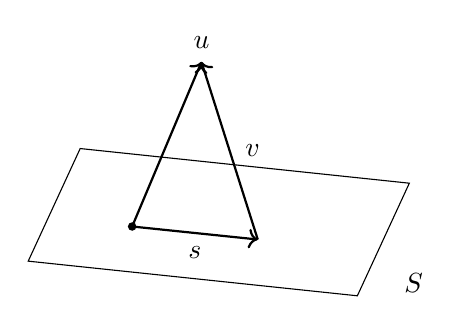
\begin{tikzpicture}[scale=1.1]
	\draw (-1.9,-0.55) -- (1.9,-0.95) -- (2.5,0.35) -- (-1.3,0.75) -- cycle;
	\node at (2.55,-0.8) {$S$};
	\coordinate (O) at (-0.7,-0.15);
	\coordinate (Sp) at (0.75,-0.3);
	\coordinate (U) at (0.1,1.75);
	\fill (O) circle (1.4pt);
	\draw[->,thick] (O) -- (Sp) node[midway,below=1pt] {$s$};
	\draw[->,thick] (O) -- (U) node[above=1pt] {$u$};
	\draw[->,thick] (Sp) -- (U) node[midway,right=2pt] {$v$};
\end{tikzpicture}
\end{center}

\begin{proof}
	Let $u \in V \setminus S$.
	Note that $\frac{d(u,S)}{1-\varepsilon} > d(u,S)$, so there exists $s \in S$ such that $\norm{u - s} < \frac{d(u,S)}{1-\varepsilon}$.
	Let $v := \frac{u-s}{\norm{u-s}}$.
	Then for $s' \in S$,
	\begin{align*}
		\norm{v - s'} = \norm{\frac{u-s}{\norm{u-s}} - s'}
		&= \frac{1}{\norm{u-s}} \norm{u - \underbrace{\left( s + s' \norm{u-s} \right)}_{\in S}} \\
		&\geq \frac{1}{\norm{u-s}} d(u,S) > 1 - \varepsilon.
	\end{align*}
	Thus $\norm{v - s'} > 1 - \varepsilon$ for all $s' \in S$, and therefore $d(v,S) \geq 1 - \varepsilon$.
\end{proof}

\begin{thm}
	Let $V$ be normed.
	Let $S_1 = \lbrace v : \norm{v} = 1 \rbrace$.
	Then $S_1$ is compact iff $V$ is finite-dimensional.
\end{thm}
\begin{proof}
	($\Leftarrow$) Real analysis.

	($\Rightarrow$) Assume $V$ is infinite-dimensional.
	Let $v_1$ be any unit vector.
	Assume $v_1, \dots, v_n$ already chosen.
	Let $v_{n+1}$ be a unit vector such that
	\begin{equation*}
		d(v_{n+1}, \spn(v_1, \dots, v_n)) > \tfrac{1}{2}.
	\end{equation*}

	\textbf{Claim: } No subsequence of $(v_n)$ converges.
	The distance between members is $> \frac{1}{2}$, so it cannot be Cauchy.
\end{proof}

\section{The Baire category theorem}

\begin{thm}[Baire Category Theorem]
	Let $F_1, F_2, F_3, \dots$ be closed sets with empty interior in a Banach space $(V, \norm{\cdot})$.
	Then $\bigcup_{i=1}^\infty F_i \neq V$.
\end{thm}
\begin{proof}
	Let $U_i = F_i^c$, so $U_i$ is open and dense for all $i$.

	\textbf{Claim: } $\bigcap_{i=1}^\infty U_i \neq \emptyset$.
	Pick $x_1 \in U_1$.
	Since $U_1$ is open, there exists $\delta_1$ such that
	\begin{enumerate}[label=(\roman*),nosep]
		\item $B_{\delta_1}(x_1) \subset U_1$,
		\item $\delta_1 < 1$.
	\end{enumerate}
	Note that $B_{\delta_1}(x_1) \cap U_2 \neq \emptyset$ and is open, so choose $x_2 \in B_{\delta_1}(x_1) \cap U_2$.
	Pick $\delta_2$ such that
	\begin{enumerate}[label=(\roman*),nosep]
		\item $\overline{B_{\delta_2}(x_2)} \subset B_{\delta_1}(x_1) \cap U_2$,
		\item $\delta_2 < \frac{1}{2}$.
	\end{enumerate}
	And so on.
	Continuing this way, we get $x_1, x_2, x_3, \dots$ such that $x_N, x_{N+1}, x_{N+2}, \dots$ lives in $B_{\delta_N}(x_N)$, so $d(x_M, x_N) < \frac{1}{N}$ for all $M > N$.
	Therefore $(x_N)$ is Cauchy, hence convergent, and there exists $x = \lim x_N$.
	Thus $x \in \overline{B_{\delta_N}(x_N)}$ for all $N$ and $\overline{B_{\delta_N}(x_N)} \subset U_N$, so
	\begin{equation*}
		x \in \bigcap_{i=1}^\infty U_i = \left( \bigcup_{i=1}^\infty F_i \right)^c. \qedhere
	\end{equation*}
\end{proof}

\begin{ex}
	$c_{00} = F_1 \cup F_2 \cup F_3 \cup \cdots$ where $F_1 = \lbrace (x_1, 0, 0, \dots) \rbrace$, $F_2 = \lbrace (x_1, x_2, 0, 0, \dots) \rbrace$, and so on.
\end{ex}

\begin{thm}
	No Banach space can have a countable Hamel basis.
\end{thm}
\begin{proof}
	Suppose $\lbrace e_i \rbrace_1^\infty$ is a countable Hamel basis.
	Define
	\begin{equation*}
		F_1 = \spn(e_1), \quad F_2 = \spn(e_1, e_2), \quad \dots
	\end{equation*}
	These are closed because they are finite-dimensional, and they have
	empty interiors.
	Therefore BCT says $\bigcup_{i=1}^\infty F_i \neq V$.
\end{proof}

\section{Dual spaces and bounded operators}

\begin{defn}
	Fix $(V, \norm{\cdot})$ over $\F$.
	Then $V^* := \lbrace f : V \to \F : f \text{ is linear \underline{and} continuous} \rbrace$ is called the \underline{dual space} of $V$ (the continuous dual).
\end{defn}

\begin{ex}
	$(\ell^p)^* = \ell^q$ where $\frac{1}{p} + \frac{1}{q} = 1$, $1 < p < \infty$.
\end{ex}

\begin{ex}
	$(\ell^1)^* = \ell^\infty$.
\end{ex}

\begin{ex}
	$(\ell^\infty)^* = \mathrm{ba}(\N)$.
\end{ex}

\begin{rmk}
	Analysts overwhelmingly care about boundedness, not continuity, because it gives you an inequality: $\abs{f e_j} \leq \abs{f} \abs{e_j}$.
	(``Michor--Kriegl convenient.'')
\end{rmk}

\begin{thm}
	For linear $f : V \to \R$, TFAE:
	\begin{enumerate}[label=(\roman*),nosep]
		\item $f$ is continuous.
		\item $f$ is continuous at $0$ ($x_n \to 0 \implies f(x_n) \to 0$).
		\item $f$ is \underline{bounded}, i.e. $\exists M \in \R$ such that $\abs{f(x)} \leq M \norm{x}$ for all $x \in V$.
		\item The preimage of open sets is open.
	\end{enumerate}
\end{thm}
\begin{proof}
	(i $\implies$ ii) Trivial.

	(ii $\implies$ iii) Suppose $f$ is not bounded.
	Then there exists $(x_n)$ such that $\abs{f(x_n)} > n \norm{x_n}$, so $\abs{f(y_n)} > n$ with $\norm{y_n} = 1$.
	Consider $z_n := \frac{y_n}{n}$.

	(iii $\implies$ iv) Let $(-\infty, b) \subset \R$.
	\textbf{Claim: } $f^{-1}((-\infty,b))$ is open.
	Let $x \in f^{-1}((-\infty,b))$, so $f(x) < b$.
	Consider
	\begin{equation*}
		f(x+y) = f(x) + f(y) \leq f(x) + \abs{f(y)} \leq f(x) + M \norm{y}.
	\end{equation*}
	Choose $\delta := \frac{b - f(x)}{M}$.
	Then if $\norm{y} \leq \delta$, we have
	\begin{equation*}
		f(x+y) < f(x) + M \left( \frac{b - f(x)}{M} \right) = b,
	\end{equation*}
	so $x + y \in f^{-1}((-\infty,b))$, and therefore $B_\delta(x) \subset f^{-1}((-\infty,b))$.

	(iv $\implies$ i) Let $(x_n)$ be a sequence with $x_n \to x$.
	We want to show that $f(x_n) \to f(x)$.
	Let $W$ be an open set containing $f(x)$.
	Let $U := f^{-1}(W)$.
	$U$ is open and $x \in U$, so $x_n \in U$ for all $n > N$.
	Therefore $f(x_n) \in W$ for all $n > N$.
\end{proof}

\begin{thm}
	For a linear $T : V_1 \to V_2$ we have an analogous theorem: $T$ continuous $\iff$ $T$ bounded.
\end{thm}

\begin{defn}
	Let $T : V_1 \to V_2$ be linear and bounded.
	The \underline{operator norm} is
	\begin{equation*}
		\norm{T}_{\mathrm{op}} = \sup_{\norm{x} \leq 1} \norm{T(x)}_{V_2} = \sup_{\norm{x} = 1} \norm{T(x)} = \sup_{x \neq 0} \frac{\norm{T(x)}}{\norm{x}}.
	\end{equation*}
\end{defn}

\begin{ex}
	The space $\cB(V_1, V_2) = \lbrace T : V_1 \to V_2 \mid T \text{ linear and bounded} \rbrace$ is normed with the operator norm.
\end{ex}

\begin{rmk}
	$\cB(V_1,V_2)$ is Banach whenever $V_2$ is Banach.
\end{rmk}

\begin{cor}
	$V^* = \cB(V,\R)$ is always Banach.
\end{cor}

\begin{ex}
	$c_{00}$ is not the dual of any space, since it isn't Banach.
\end{ex}

\begin{rmk}
	Two normed spaces $V_1, V_2$ are \underline{isomorphic} if there exists a bijective bounded linear map such that its inverse is also bounded.
	If $\norm{T(x)}_{V_2} = \norm{x}_{V_1}$, then $V_1$ and $V_2$ are \underline{isometric}.
\end{rmk}

\begin{thm}
	$(\ell^1)^* \cong \ell^\infty$.
\end{thm}
\begin{proof}
	Let
	\begin{align*}
		\varphi : \ell^\infty &\to (\ell^1)^* \\
		x &\mapsto \varphi(x) : \ell^1 \to \R \\
		&\qquad\quad\ y \mapsto \sum_{j=1}^\infty x_j y_j.
	\end{align*}

	\textbf{Claim: } $\varphi(x)$ is bounded, i.e. $\varphi(x) \in (\ell^1)^*$.
	\begin{equation*}
		\abs{\varphi(x)(y)} = \abs{\sum x_j y_j} \leq \sum \abs{x_j y_j} \leq \sum \norm{x}_\infty \abs{y_j} = \norm{x}_\infty \sum \abs{y_j} = \norm{x}_\infty \norm{y}_1.
	\end{equation*}
	Therefore $\abs{\varphi(x)(y)} \leq \norm{x}_\infty \norm{y}_1$.
	In particular, $\sup_{\norm{y}_1 \leq 1} \abs{\varphi(x)(y)} \leq \norm{x}_\infty$.

	\textbf{Claim: } $\norm{\varphi(x)}_{\mathrm{op}} = \norm{x}_\infty$.
	We already have $\leq$.
	Let $x = (x_1, x_2, \dots) \in \ell^\infty$.
	Note $\abs{\varphi(x)(e_j)} = \abs{x_j} \leq \norm{\varphi(x)}_{\mathrm{op}}$, so $\norm{x}_\infty \leq \norm{\varphi(x)}_{\mathrm{op}}$.

	Note: if $\varphi(x) = 0$, then $\norm{\varphi(x)}_{\mathrm{op}} = 0$, so $\varphi$ is injective.

	\textbf{Claim: } $\varphi$ is surjective.
	Let $f : \ell^1 \to \R$ be bounded linear.
	Define $x_j := f(e_j)$.
	Then $\varphi(x) = f$.
	Note that $\abs{x_j} = \abs{f(e_j)} \leq \norm{f}_{\mathrm{op}} \norm{e_j}_1 = \norm{f}_{\mathrm{op}}$, so $x \in \ell^\infty$.
	To show $\varphi(x) = f$, let $y \in c_{00} \subset \ell^1$:
	\begin{align*}
		\varphi(x)(y) &= x_1 y_1 + \cdots + x_N y_N = f(e_1) y_1 + \cdots + f(e_N) y_N \\
		&= f(y_1 e_1 + \cdots + y_N e_N) = f(y).
	\end{align*}
	So they match on a dense subspace ($c_{00}$), and therefore they match everywhere by continuity.
\end{proof}

\begin{rmk}[Density argument]
	If $\varphi(x)(y) = f(y)$ for all $y \in c_{00}$ (dense), let $z \in \ell^1$ with $z_n \to z$, $z_n \in c_{00}$.
	Then
	\begin{equation*}
		\varphi(x)(z_n) = f(z_n) \xrightarrow{\ n \to \infty\ } \varphi(x)(z) = f(z).
	\end{equation*}
	This is an important argument in analysis, called a ``density argument.''
\end{rmk}

\section{Extension of functionals and Hahn--Banach}

\begin{rmk}
	Can we do it on a dense set?
	You can extend any linearly independent set to a Hamel basis.
\end{rmk}

\begin{lma}
	Let $D \subset V$ be a dense subspace.
	Given a bounded linear functional $f : D \to \R$, there exists a unique extension of $f$ to $V$ given by
	\begin{align*}
		\tilde{f} &: V \to \R \\
		\tilde{f}(v) &= \lim_{n \to \infty} f(v_n) \quad \text{where } v_n \to v, \ v_n \in D.
	\end{align*}
	Furthermore, $\norm{\tilde{f}}_{\mathrm{op}} = \norm{f}_{\mathrm{op}}$.
\end{lma}
\begin{proof}
	Suppose $(v_n), (v_n')$ are sequences in $D$ both converging to $v$.
	Then
	\begin{equation*}
		\abs{f(v_n) - f(v_n')} = \abs{f(v_n - v_n')} \leq \norm{f}_{\mathrm{op}} \norm{v_n - v_n'} \leq \norm{f}_{\mathrm{op}} \left( \norm{v_n - v} + \norm{v - v_n'} \right) \to 0.
	\end{equation*}
	Also
	\begin{equation*}
		\tilde{f}(v+w) = \lim f(v_n + w_n) = \lim f(v_n) + \lim f(w_n) = \tilde{f}(v) + \tilde{f}(w). \qedhere
	\end{equation*}
\end{proof}

\begin{ex}
	Given $f : \R \to \R$ continuous with compact support,
	\begin{equation*}
		\hat{f}(\xi) := \int_{-\infty}^\infty f(x) e^{2\pi i x \xi} \, dx
	\end{equation*}
	is well defined.
	Here $\widehat{\ \cdot\ } : C^0_{cs}(\R) \to C^0(\R)$ and $\norm{\hat{f}}_{L^2} = \norm{f}_{L^2}$.
\end{ex}

\begin{ex}
	$c_{00}$ is dense in $\ell^1$.
	Define $f : c_{00} \to \R$ by $f(\underbrace{(0,0,\dots,1,\dots,0,\dots)}_{e_i}) = 1$, where $c_{00} = \spn\lbrace e_1, e_2, \dots \rbrace$.

	\textbf{Claim: } $f$ is bounded as a functional on $(c_{00}, \norm{\cdot}_{\ell^1})$.
	Let $\norm{x}_{\ell^1} = 1$.
	This means $\sum_1^N \abs{x_i} = 1$, so
	\begin{equation*}
		\abs{f(x)} = \abs{f(x_1, x_2, \dots, x_N, 0, \dots)} = \abs{\sum_1^N x_i f(e_i)} \leq 1,
	\end{equation*}
	and therefore $\norm{f}_{\mathrm{op}} \leq 1$.
	\begin{enumerate}[label=(\roman*)]
		\item We can extend to $\ell^1$: $\tilde{f} : \ell^1 \to \R$,
		\begin{equation*}
			\tilde{f}((x_1,x_2,\dots)) = \lim_n f(x_1, x_2, \dots, x_n, 0, 0, \dots) = \lim_n \sum_1^n x_i = \sum_1^\infty x_i.
		\end{equation*}
		\item Let $e = (1, \tfrac{1}{2}, \tfrac{1}{4}, \dots) \in \ell^1$, $e \notin c_{00}$.
		Take $\lbrace e_i \rbrace_1^\infty \cup \lbrace e \rbrace \cup A = B \approx$ Hamel.
		Define $\tilde{f} : \ell^1 \to \R$ by $\tilde{f}(e) = 0$, $\tilde{f}(a) = 0$ for all $a \in A$.
		\textbf{Claim: } $f$ is unbounded.
	\end{enumerate}
\end{ex}

\begin{ex}
	Let $f : \R(1,1) \to \R$ (the span of $(1,1)$) be given by $f(x,x) = x$.
	Define $\tilde{f} : \R(1,1) \oplus \R(0,1) \to \R$ by making $\tilde{f}|_{\R(0,1)} = 0$.
	Then
	\begin{equation*}
		\norm{f}_{\mathrm{op}} = \sup_{\norm{(x,x)}=1} \abs{f(x,x)} = \sup_{x^2 + x^2 = 1} \abs{x} = \frac{1}{\sqrt{2}} < 1,
	\end{equation*}
	while $\tilde{f}(x,y) = \tilde{f}((x,x) + (0,y-x)) = \tilde{f}(x,x) + \tilde{f}(0,y-x) = x$, so
	\begin{equation*}
		\norm{\tilde{f}}_{\mathrm{op}} = \sup_{\norm{(x,y)}=1} \abs{\tilde{f}(x,y)} = \sup_{\norm{(x,y)}=1} \abs{x} = 1.
	\end{equation*}
	Moral: extending by zeroes may not increase $\norm{\cdot}_{\mathrm{op}}$.
	\begin{center}
	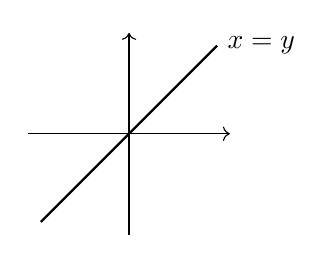
\begin{tikzpicture}[scale=0.8]
		\draw[->] (-1.6,0) -- (1.6,0);
		\draw[->] (0,-1.6) -- (0,1.6);
		\draw[thick] (-1.4,-1.4) -- (1.4,1.4) node[right] {$x=y$};
	\end{tikzpicture}
	\end{center}
\end{ex}

\begin{thm}[Hahn--Banach]
	Let $V$ be a normed space and $S$ a subspace, not necessarily dense.
	Then given a bounded linear functional $f : S \to \R$, there exists an extension $\hat{f} : V \to \R$ with $\norm{\hat{f}}_{\mathrm{op}} = \norm{f}_{\mathrm{op}}$.
\end{thm}
\begin{proof}
	\textbf{Claim: } Let $v \in V \setminus S$.
	Then there exists an extension $\tilde{f} : S \oplus \R v \to \R$ with $\norm{\tilde{f}}_{\mathrm{op}} \leq \norm{f}_{\mathrm{op}}$.

	The goal is to choose $\alpha = \tilde{f}(v)$ such that the norm doesn't increase:
	\begin{equation*}
		\abs{\tilde{f}(s + \lambda v)} \leq C \norm{s + \lambda v}, \quad \forall s \in S, \lambda \in \R.
	\end{equation*}
	(Divide by $\abs{\lambda}$.)
	Equivalently, $\abs{\tilde{f}(s \pm v)} \leq C \norm{s \pm v}$ for all $s \in S$; equivalently
	\begin{equation*}
		\begin{cases}
			\tilde{f}(s+v) \leq C \norm{s+v} \\
			\tilde{f}(s-v) \leq C \norm{s-v}
		\end{cases} \forall s \in S;
	\end{equation*}
	equivalently
	\begin{equation*}
		\begin{cases}
			\alpha \leq C \norm{s+v} - f(s) \\
			-\alpha \leq C \norm{s-v} - f(s) \iff \alpha \geq f(s) - C \norm{s-v}
		\end{cases} \forall s \in S.
	\end{equation*}
	WTS:
	\begin{equation*}
		\sup_{s \in S} f(s) - C \norm{s - v} \leq \inf_{s \in S} C \norm{s+v} - f(s).
	\end{equation*}
	So $f(s') - C\norm{s' - v} \leq C \norm{s+v} - f(s)$, i.e.
	\begin{equation*}
		f(s' + s) \leq C \left( \norm{s+v} + \norm{s'-v} \right). \tag{$\star$}
	\end{equation*}
	Proof of $(\star)$:
	\begin{equation*}
		f(\underbrace{s + s'}_{\in S}) \leq C \norm{s+s'} = C \norm{s + v - v + s'} \leq C \left( \norm{s+v} + \norm{s'-v} \right).
	\end{equation*}

	Now let $X = \lbrace$ all extensions of $f : S \to \R$ with norm $\leq \norm{f}_{\mathrm{op}} \rbrace$, ordered by inclusion:
	\begin{equation*}
		(\tilde{f}, S \oplus z) \ \nwarrow\ (f,S) \ \nearrow\ (\hat{f}, S \oplus \omega).
	\end{equation*}
	Each chain has an upper bound $\bigcup f_i$.
	Use Zorn, so that there is a maximal element, and it must be on the whole space, because if it weren't we could just add one dimension.
\end{proof}

\begin{lma}[Zorn's]
	Let $(X, \leq)$ be a poset.
	If every chain in $X$ has an upper bound, then $X$ has a maximal element.
\end{lma}

\section{Convexity and Krein--Milman}

\begin{thm}[Geometric Hahn--Banach]
	Let $(V, \norm{\cdot})$ be a normed space, $F$ a closed, convex, nonempty subset of $V$, and $z \notin F$.
	Then there exists $f \in V^*$ such that $f(x) \leq c \leq f(z)$ for all $x \in F$, for some $c \in \R$.
\end{thm}

\begin{center}
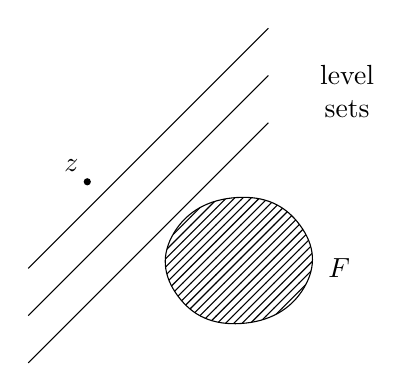
\begin{tikzpicture}[scale=1.0]
	\draw[pattern=north east lines] plot[smooth cycle,tension=0.8]
		coordinates {(0.15,0.15) (0.95,-0.2) (1.0,-1.0) (0.2,-1.45) (-0.6,-1.1) (-0.65,-0.3)};
	\node at (1.45,-0.75) {$F$};
	\foreach \c in {0.55,1.15,1.75}{%
		\draw (-2.5,-2.5+\c) -- (0.55,0.55+\c);}
	\fill (-1.75,0.35) circle (1.3pt);
	\node at (-1.95,0.55) {$z$};
	\node[align=center] at (1.55,1.5) {level\\ sets};
\end{tikzpicture}
\end{center}

\begin{defn}
	A \underline{convex combination} of $v_1, \dots, v_n$ is $\lambda_1 v_1 + \cdots + \lambda_n v_n$ so that $\sum_1^n \lambda_i = 1$, each $\lambda_i \geq 0$.
\end{defn}

\begin{defn}
	Given $A \subset V$, the \underline{convex hull} of $A$ is $\conv(A)$, the set of convex combinations of elements of $A$.
\end{defn}

\begin{defn}
	$A \subset V$ is \underline{convex} if $A = \conv(A)$.
\end{defn}

\begin{defn}
	Let $C$ be a convex set.
	A subset $F \subset C$ is a \underline{face} of $C$ if $F$ is closed, nonempty, and if for $x, y \in C$, whenever there exists $t_0 \in (0,1)$ such that $t_0 x + (1-t_0) y \in F$, then $[x,y] \subset F$.
\end{defn}

\begin{defn}
	An \underline{extreme point} of $C$ is a face with one element.
\end{defn}

\begin{defn}
	Let $x, y \in V$.
	Then we write
	\begin{align*}
		(x,y) &= \lbrace tx + (1-t)y : t \in (0,1) \rbrace, \\
		[x,y] &= \lbrace tx + (1-t)y : t \in [0,1] \rbrace.
	\end{align*}
\end{defn}

\begin{lma}
	If $F'$ is a face of $F$ and $F$ is a face of $C$, then $F'$ is a face of $C$.
\end{lma}

\begin{thm}[Krein--Milman]
	Let $K$ be a compact, convex, nonempty subset $K \subset V$.
	Then $K = \overline{\conv(\Ext(K))}$, where $\Ext(K) = \lbrace$ extreme points of $K \rbrace$.
\end{thm}
\begin{proof}
	\textbf{Claim: } $\Ext(K)$ is nonempty.

	Let $J := \lbrace$ all faces of $K \rbrace$.
	Order $J$ by reverse inclusion.
	Suppose $\lbrace F_\alpha \rbrace_\alpha$ is a chain in $J$.
	Take $F := \bigcap_\alpha F_\alpha$.
	Then $F \supseteq F_\alpha$ for all $\alpha$ in this order.
	That $F$ is closed follows by each $F_\alpha$ being closed.
	Likewise for convexity and the ``face'' condition.
	We need to argue nonemptiness.
	If $F$ were empty, $K = F^c = \bigcup F_\alpha^c$, and each $F_\alpha^c$ is open, so this would be an open cover of $K$ with no finite subcover.
	Therefore Zorn's Lemma says there exists a maximal element $F_0 \in J$.

	\textbf{Subclaim: } Any minimal/maximal $F_0 \in J$ is a singleton.
	Suppose not, so $x, y \in F_0$, $x \neq y$.
	By Hahn--Banach there exists $f \in V^*$ such that $f(x) \neq f(y)$.
	The function $g = f|_{F_0} : F_0 \to \R$ is continuous and $F_0$ is compact, so $g$ obtains a maximum $M$.
	Take $F_1 = g^{-1}(M) = \lbrace x \in F_0 : g(x) = M \rbrace$.
	But $F_1$ is a face of $F_0$ (thus of $K$), because it's the preimage of a singleton and so closed; it's nonempty by construction; and if $z, \omega \in F_0$ and $t \in (0,1)$ with $tz + (1-t)\omega \in F_1$, then $g(tz + (1-t)\omega) = t g(z) + (1-t) g(\omega) = M$, and since $g(z) \leq M$ and $g(\omega) \leq M$, we get $g(z) = g(\omega) = M$, so $z, \omega \in F_1$; and it is convex because it's a level set.

	\begin{center}
	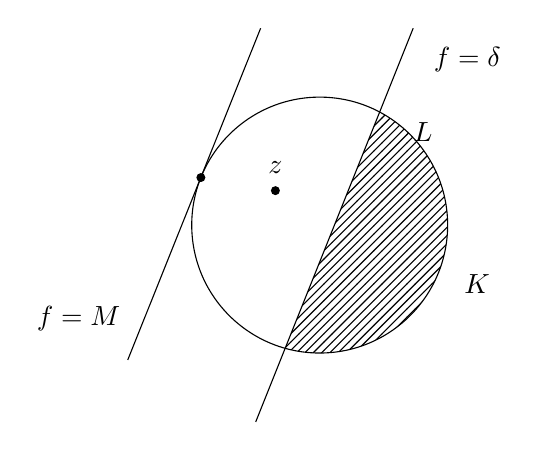
\begin{tikzpicture}[scale=1.25]
		\begin{scope}
			\clip (0,0) circle (1.3);
			\fill[pattern=north east lines] (-0.65,-2) -- (0.95,2) -- (3,2) -- (3,-2) -- cycle;
		\end{scope}
		\draw (0,0) circle (1.3);
		\draw (-0.65,-2) -- (0.95,2);
		\node at (1.5,1.68) {$f=\delta$};
		\draw (-1.95,-1.37) -- (-0.6,2.00);
		\node at (-2.45,-0.95) {$f=M$};
		\fill (-1.207,0.483) circle (1.3pt);
		\fill (-0.45,0.35) circle (1.3pt);
		\node at (-0.45,0.58) {$z$};
		\node at (1.05,0.95) {$L$};
		\node at (1.6,-0.6) {$K$};
	\end{tikzpicture}
	\end{center}

	We've shown that $\Ext(K) \neq \emptyset$.
	Let $L = \overline{\conv(\Ext(K))}$.
	Suppose that $K \setminus L \neq \emptyset$.
	Pick $z \in K \setminus L$.
	By geometric Hahn--Banach, there exists $f \in V^*$ such that $f(z) > \delta \geq f(x)$ for all $x \in L$.
	Maximize $f$ over $K$; let the max be $M$.
	Note that $F_0 := f^{-1}(M)$ does not intersect $L$.
	But $F_0$ is a face, so by the Zorn's Lemma argument from before, it contains an extreme point.
\end{proof}

\section{The open mapping and closed graph theorems}

\begin{thm}[Open mapping theorem]
	Let $T : X \to Y$ be linear, bounded, and surjective, where $X, Y$ are Banach.
	Then $T$ is an open map.
\end{thm}
\begin{proof}
	Note that $\bigcup_{n=1}^\infty \overline{T(B_n^X(0))} = Y$.
	By BCT, there exists $N$ such that $\overline{T(B_N^X(0))}$ has nonempty interior.
	Therefore there exists $B_r^Y(y_0) \subset \overline{T(B_N^X(0))}$.

	\textbf{Claim: } $\overline{T(B_N^X(0))}$ contains a ball centered at $0$.
	Take $y \in Y$ with $\norm{y} < r$.
	Then $y_0 \in \overline{T(B_N^X(0))}$ and $y_0 + y \in \overline{T(B_N^X(0))}$, so
	\begin{equation*}
		\left.
		\begin{aligned}
			\exists (x_n) \subset B_N^X(0) \text{ s.t. } T(x_n) &\to y_0 \\
			\exists (x_n') \subset B_N^X(0) \text{ s.t. } T(x_n') &\to y_0 + y
		\end{aligned}
		\right\rbrace \implies T(x_n' - x_n) \to y.
	\end{equation*}
	Note $x_n' - x_n \in B_{2N}^X(0)$, so $y \in \overline{T(B_{2N}^X(0))}$.
	So $B_r^Y(0) \subset \overline{T(B_{2N}^X(0))}$, and therefore $B_{r/2}^Y(0) \subset \overline{T(B_N^X(0))}$.

	(Here $\tfrac{1}{2}\overline{A} = \overline{\tfrac{1}{2}A}$, because multiplication by half is a homeomorphism, so $m(\overline{A}) = \overline{m(A)}$.)

	By rescaling, we have $B_1^Y(0) \subset \overline{T(B_\delta^X(0))}$.
	Let $y \in B_1^Y(0)$.
	Since $y \in \overline{T(B_\delta^X(0))}$,
	\begin{align*}
		&\exists x_1 \in B_\delta^X(0) \text{ s.t. } \norm{y - T(x_1)} < \tfrac{1}{2} \\
		&\exists x_2 \in B_{\delta/2}^X(0) \text{ s.t. } \norm{y - T(x_1) - T(x_2)} < \tfrac{1}{4} \\
		&\exists x_3 \in B_{\delta/4}^X(0) \text{ s.t. } \norm{y - T(x_1) - T(x_2) - T(x_3)} < \tfrac{1}{8} \\
		&\quad \vdots \\
		&\exists x_n \in B_{\delta/2^{n-1}}^X(0) \text{ s.t. } \norm{y - \sum_{i=1}^n T(x_i)} < \tfrac{1}{2^n}.
	\end{align*}
	Note $\sum_{i=1}^\infty \norm{x_i} < 2\delta$.
	Absolute convergence implies convergence, so $x = \sum_{i=1}^\infty x_i \in X$.
	Continuity of $T$ then gives $T(x) = y$.
	(Tip: to move a limit inside, use continuity.)
	Also $\norm{x} \leq \sum_{i=1}^\infty \norm{x_i} < 2\delta$, so
	\begin{equation*}
		B_1^Y(0) \subset T(B_{2\delta}^X(0)). \tag{$\star$}
	\end{equation*}
	$(\star)$ implies that $T(B_\varepsilon^X(0)) \supset B_{\varepsilon'}^Y(0)$ (for all $\varepsilon$ there exists $\varepsilon'$).
	This implies that for all $\varepsilon > 0$ there exists $\varepsilon' > 0$ such that for all $x_0 \in X$, $T(B_\varepsilon^X(x_0)) \supset B_{\varepsilon'}^Y(T(x_0))$:
	\begin{align*}
		T(x_0) + T(B_\varepsilon^X(0)) &\supset B_{\varepsilon'}^Y(0) + T(x_0) \\
		T(B_\varepsilon^X(0) + x_0) &\supset B_{\varepsilon'}^Y(T(x_0)) \\
		T(B_\varepsilon^X(x_0)) &\supset B_{\varepsilon'}^Y(T(x_0)).
	\end{align*}
	Therefore $T$ is open.
\end{proof}

\begin{cor}
	If $T : X \to Y$ is bounded, linear, and bijective, with $X, Y$ Banach, then $T$ is an isomorphism.
\end{cor}

\begin{thm}[Closed graph theorem]
	Let $X, Y$ be Banach and $T : X \to Y$ linear.
	Then $T$ is bounded iff $G(T) = \lbrace (x, T(x)) : x \in X \rbrace \subseteq X \times Y$ is closed.
	Note $G(T) \cong T$, and $\norm{(x,y)} = \norm{x} + \norm{y}$.
\end{thm}
\begin{proof}
	($\Rightarrow$) Immediate.

	($\Leftarrow$) $G(T) \subset X \times Y$ is a closed subspace, therefore Banach on its own.
	We have
	\begin{align*}
		\pi_1 : G(T) &\to X & \varphi : X &\to G(T) \\
		(x, T(x)) &\mapsto x & x &\mapsto (x, T(x)).
	\end{align*}
	$\pi_1, \varphi$ are linear and $\pi_1 = \varphi^{-1}$.
	But $\pi_1$ is bounded:
	\begin{equation*}
		\norm{\pi_1(x,y)} = \norm{x} \leq \norm{x} + \norm{y}.
	\end{equation*}
	Therefore $\varphi$ is also bounded by the OMT corollary, and $T = \pi_2 \circ \varphi$, so $T$ is bounded by composition.
\end{proof}

\section{Recap}

\begin{equation*}
	\underbrace{\text{B.C.T.}}_{\text{completeness}}
	\begin{cases}
		\longrightarrow \text{Open mapping} \\
		\longrightarrow \text{Closed graph} \\
		\longrightarrow \text{Uniform boundedness (Banach--Steinhaus)}
	\end{cases}
\end{equation*}

\begin{itemize}
	\item \textbf{OMT: } $X, Y$ Banach, $T : X \to Y$ linear, surjective, bounded $\implies T$ open.
	\item \textbf{CGT: } $X, Y$ Banach, $T : X \to Y$ linear; $T$ bounded $\iff \lbrace (x, T(x)) \rbrace$ closed.
	\item \textbf{UBT: } $\lbrace T_\alpha : X \to Y, \text{ bounded} \rbrace_{\alpha \in J}$; $\sup_\alpha \norm{T_\alpha(x)} < \infty$ for all $x$ $\implies \sup_\alpha \norm{T_\alpha}_{\mathrm{op}} < \infty$.
	\item Hahn--Banach $\implies$ Krein--Milman.
\end{itemize}

\section{Projections}

\begin{defn}
	A linear map $P$ is called a \underline{projection} if $P^2 = P \circ P = P$.
\end{defn}

\begin{thm}
	Let $X$ be a Banach space.
	Let $Y$ be a closed, complemented subspace (i.e.\ there exists $Z \subset X$ a closed subspace such that $X = Y \oplus Z$).
	Define $P : X \to Y \oplus Z$, $x \mapsto (y,0)$.
	Then $P$ is a projection and it is bounded.
\end{thm}
\begin{proof}
	Projection: obvious.
	To see that $P$ is bounded, use CGT.
	Assume $\underbrace{(x_n, P(x_n))}_{\in X \times Y} \to \underbrace{(x,y)}_{\in X \times Y}$.
	WTS: $y = P(x)$.
	Note
	\begin{equation*}
		(1-P)(x) = (y,z) - P(x) = (y,z) - (y,0) = (0,z),
	\end{equation*}
	and
	\begin{equation*}
		x_n = \underbrace{Px_n}_{\downarrow} + \underbrace{(1-P)x_n}_{\downarrow}, \qquad x = \underbrace{y}_{\in Y} + \underbrace{(x-y)}_{\in Z}.
	\end{equation*}
	Therefore $x - y \in Z = \ker(P)$, so $P(x-y) = 0$, giving $P(x) = P(y) = y$.
\end{proof}

\section{Spectrum of an operator}

Given $T : X \to X$, the question is: is $T - \lambda \Id$ invertible, $\lambda \in \C$?
(Think of $T - \lambda \Id$ as a tiny perturbation.)
The answer is: very often.

\begin{ex}
	$T = \begin{pmatrix} 3 & 0 \\ 0 & 5 \end{pmatrix} : \R^2 \to \R^2$.
	When is $T - \lambda$ invertible?
	Any $\lambda \neq 3$ or $5$.
	Therefore $\underbrace{\sigma(T)}_{\text{spectrum}} = \lbrace 3, 5 \rbrace$ and $\underbrace{\rho(T)}_{\text{resolvent}} = \C \setminus \lbrace 3, 5 \rbrace$.
\end{ex}

\begin{ex}
	$T = \begin{pmatrix} 3 & 2 \\ 2 & 3 \end{pmatrix}$, $\sigma(T) = \lbrace 1, 5 \rbrace$, since
	\begin{equation*}
		\det(T - \lambda) = 0 = (3-\lambda)^2 - 4.
	\end{equation*}
\end{ex}

\begin{rmk}
	Rank-nullity: for $T : \R^n \to \R^n$, $\dim \ker(T) + \dim \im(T) = n$.
\end{rmk}

\begin{defn}
	Let $T : X \to X$ be bounded, $X$ Banach.
	Then $\lambda \in \C$ is in the \underline{spectrum} of $T$ if $(T-\lambda)^{-1} : X \to X$ is not in $\cB(X,X)$.
	This can fail for different reasons:
	\begin{enumerate}[nosep]
		\item If $T - \lambda$ has a kernel, we say $\lambda \in \sigma_p(T)$ (\underline{point spectrum}).
		\item If $T - \lambda$ is injective but not surjective, and $\Im(T-\lambda)$ is dense, then $\lambda \in \sigma_c(T)$ (\underline{continuous spectrum}).
		\item If $T - \lambda$ is injective but $\Im(T - \lambda)$ is \underline{not} dense, then $\lambda \in \sigma_r(T)$ (\underline{residual spectrum}).
	\end{enumerate}
\end{defn}

\noindent In case (2), $(T-\lambda)^{-1} : D \subset X \to X$ exists, but \underline{must} be unbounded, since you can continuously extend from a dense subset.
Therefore
\begin{equation*}
	\sigma(T) = \sigma_p(T) \sqcup \sigma_c(T) \sqcup \sigma_r(T), \qquad \C \setminus \sigma(T) = \rho(T) \ (\text{resolvent}).
\end{equation*}

\begin{ex}
	$M : C^0[a,b] \to C^0[a,b]$, $f \mapsto Mf$, where $(Mf)(t) = t f(t)$.

	$M$ is linear:
	\begin{equation*}
		(M(f_1 + f_2))(t) = t(f_1(t) + f_2(t)) = (Mf_1 + Mf_2)(t).
	\end{equation*}
	$M$ is bounded:
	\begin{equation*}
		\abs{(Mf)(t)} = \abs{t f(t)} \leq \abs{t} \norm{f(t)}_\infty \leq \abs{t} \leq \abs{b}.
	\end{equation*}
	Any $f \in C^0[a,b]$, $f \neq 0$, such that $Mf = \lambda f$ satisfies
	\begin{align*}
		(Mf)(t) &= \lambda f(t) \quad \forall t \\
		t f(t) &= \lambda f(t) \\
		(t - \lambda) f(t) &= 0 \quad \forall t \\
		\implies f &= 0.
	\end{align*}

	\textbf{Claim: } If $\lambda \notin [0,1]$, then $\lambda \in \rho(M)$ (taking $[a,b] = [0,1]$).
	Given $g \in C^0[0,1]$, consider
	\begin{equation*}
		(M - \lambda) f = g \iff (t-\lambda) f(t) = g(t) \quad \forall t \in [0,1].
	\end{equation*}
	We can solve this by setting $f(t) = \frac{g(t)}{t - \lambda}$.
	Therefore $\sigma(M) \subset [0,1]$.

	If $\lambda \in [0,1]$, e.g.\ $\lambda = \frac{1}{2}$, then
	\begin{equation*}
		\Im\left( M - \tfrac{1}{2} \right) \subset \left\lbrace f \in C^0[0,1] : f\left( \tfrac{1}{2} \right) = 0 \right\rbrace,
	\end{equation*}
	which cannot be dense in $C^0[0,1]$.
	So $\frac{1}{2} \in \sigma_r(M)$.
	Similarly, $[0,1] \subset \sigma_r(M)$, and thus $\sigma(M) = [0,1]$.
\end{ex}

\begin{thm}
	For any $T \in \cB(X)$, $\sigma(T)$ is a compact, nonempty subset of $\C$.
	Furthermore, $\sigma(T) \subset B_{\norm{T}_{\mathrm{op}}}[0]$.
\end{thm}

\begin{rmk}
	Compactness comes from Calc 2; nonemptiness comes from the physics of the heat equation.
\end{rmk}

\begin{ex}[Left shift]
	$L : \ell^2 \to \ell^2$, $L(x_1, x_2, x_3, \dots) = (x_2, x_3, x_4, \dots)$.
	\begin{equation*}
		(L - \lambda)(x) = 0 \implies (x_2 - \lambda x_1, x_3 - \lambda x_2, \dots) = 0 \tag{E}
	\end{equation*}
	gives $x_2 = \lambda x_1$, $x_3 = \lambda x_2 = \lambda^2 x_1, \dots$.
	Solutions of (E) are of the form $x_1(1, \lambda, \lambda^2, \lambda^3, \dots)$.
	Every $\abs{\lambda} < 1$ gives an eigenvector, i.e.\ $(1, \lambda, \lambda^2, \dots)$.
	\begin{center}
	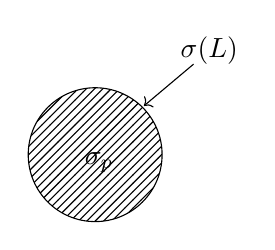
\begin{tikzpicture}[scale=1.0]
		\draw[pattern=north east lines] (0,0) circle (0.85);
		\node at (0.05,-0.1) {$\sigma_p$};
		\draw[->] (1.25,1.15) -- (0.62,0.62);
		\node at (1.45,1.32) {$\sigma(L)$};
	\end{tikzpicture}
	\end{center}
	Consider now $\abs{\lambda} = 1$.
	Then $\lambda \notin \sigma_p(L)$.

	\textbf{Q: } Is $\Im(L - \lambda)$ dense?
	Consider $\lambda = 1$.
	Then $(L-1)(x) = (x_2 - x_1, x_3 - x_2, \dots)$.
	Given $(y_1, y_2, \dots, y_N, 0, \dots) = y$, we claim that $(L-1)(x) = y$ is solvable:
	$y_1 = x_2 - x_1$, $y_2 = x_3 - x_2, \dots, y_N = x_{N+1} - x_N$.
	This is solvable, so $\Im(L-1)$ is dense.
\end{ex}

\begin{lma}
	If $\norm{T}_{\mathrm{op}} < 1$, then $1 - T$ is invertible.
\end{lma}
\begin{proof}
	\begin{equation*}
		(1-T) \underbrace{\left( 1 + T + T^2 + \cdots + T^N \right)}_{S_N(T)} = 1 - T^{N+1}. \tag{$\star$}
	\end{equation*}
	Note that $\sum_{n=0}^\infty \norm{T}_{\mathrm{op}}^n < \infty$, so $\sum_{n=0}^\infty T^n$ converges, i.e.\ $S_N(T)$ converges to some operator $S$.
	Taking limits in $(\star)$, we get $(1-T) S = 1$.
\end{proof}

\begin{thm}
	For $T \in \cB(X)$, $\rho(T)$ is open in $\C$.
\end{thm}
\begin{proof}
	Fix $\lambda_0 \in \rho(T)$, so $T - \lambda_0$ is invertible.
	\begin{equation*}
		T - \lambda = T - \lambda_0 - (\lambda - \lambda_0) = (T - \lambda_0) \left( 1 - \underbrace{(\lambda - \lambda_0)(T-\lambda_0)^{-1}}_{R} \right),
	\end{equation*}
	and
	\begin{equation*}
		\norm{(\lambda - \lambda_0)(T - \lambda_0)^{-1}}_{\mathrm{op}} = \abs{\lambda - \lambda_0} \cdot \norm{(T-\lambda_0)^{-1}}_{\mathrm{op}}.
	\end{equation*}
	As long as $\abs{\lambda - \lambda_0} < \frac{1}{\norm{(T-\lambda_0)^{-1}}_{\mathrm{op}}}$, $1 - R$ is invertible by the Lemma.
\end{proof}

\begin{thm}
	$\sigma(T) \subset B_{\norm{T}_{\mathrm{op}}}[0]$.
\end{thm}
\begin{proof}
	Suppose $\abs{\lambda} > \norm{T}_{\mathrm{op}}$.
	Then
	\begin{equation*}
		T - \lambda = \lambda \left( \tfrac{T}{\lambda} - 1 \right) = -\lambda \left( 1 - \tfrac{T}{\lambda} \right),
	\end{equation*}
	and $\norm{\frac{T}{\lambda}}_{\mathrm{op}} = \frac{1}{\abs{\lambda}} \norm{T}_{\mathrm{op}} < 1$, so $1 - \frac{T}{\lambda}$ is invertible.
\end{proof}

\begin{rmk}
	$\cB(\ell^1) \xrightarrow{\ \sigma\ } 2^\C$, with $\Im(\sigma) = $ all compact subsets.
\end{rmk}

\section{The heat equation}

Principle: heat flows from hot to cold.
\begin{align*}
	\text{1D: } &u_t = u_{xx} \\
	\text{2D: } &u_t = u_{xx} + u_{yy}
\end{align*}
$\Delta u = u_{xx} + u_{yy}$ is the Laplacian.
The general heat equation is $u_t = \Delta u$, where $\Delta$ reads (average of values in a neighborhood of $x$) $- \, u(x)$.
\begin{itemize}[nosep]
	\item If $\Delta u > 0$, neighbors are warmer.
	\item If $\Delta u < 0$, neighbors are cooler.
	\item If $\Delta u \equiv 0$, $u$ is harmonic, and is called an \underline{equilibrium solution}.
\end{itemize}

\begin{ex}
	$u(x,y) = y^2 - x^2$.
\end{ex}

\noindent But how can you have a solution where heat is different everywhere forever, since heat is supposed to equal out?
Answer: there are infinite heat sinks along the $y$-axis and cool sinks on the $x$-axis.
We need to restrict.

\begin{thm}[Liouville's, first form]
	A bounded, harmonic function on the whole plane is constant.
\end{thm}

\section{Complex analysis}

Complex analysis is about steady solutions to the heat equation.

\begin{defn}
	The complex derivative is
	\begin{equation*}
		f'(z) = \lim_{\omega \to z} \frac{f(z) - f(\omega)}{z - \omega}.
	\end{equation*}
\end{defn}

\noindent $f(z) = \bar{z}$ is not complex differentiable anywhere.

\begin{defn}
	$f : \C \to \C$ is \underline{analytic} if it is complex differentiable everywhere.
\end{defn}

\noindent Analytic $\iff \mathrm{Re}_x = \mathrm{Im}_y$, $\mathrm{Re}_y = -\mathrm{Im}_x$.
So every analytic function has harmonic real and imaginary parts.

\subsection*{Line integrals}

A curve is $\gamma : [a,b] \to \C$, and
\begin{equation*}
	\int_\gamma f(z) \, dz := \lim_{\norm{P} \to 0} \sum_k (z_{k+1} - z_k) f(z_k).
\end{equation*}
\begin{center}
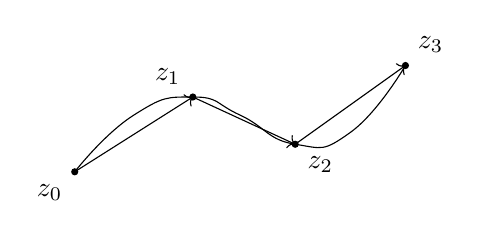
\begin{tikzpicture}[scale=1.0]
	\coordinate (z0) at (0,0);
	\coordinate (z1) at (1.5,0.95);
	\coordinate (z2) at (2.8,0.35);
	\coordinate (z3) at (4.2,1.35);
	\draw plot[smooth,tension=0.9] coordinates {(z0) (0.75,0.72) (z1) (2.1,0.72) (z2) (3.5,0.5) (z3)};
	\draw[->] (z0) -- (z1);
	\draw[->] (z1) -- (z2);
	\draw[->] (z2) -- (z3);
	\foreach \p in {z0,z1,z2,z3}{\fill (\p) circle (1.3pt);}
	\node[below left=1pt] at (z0) {$z_0$};
	\node[above left=1pt] at (z1) {$z_1$};
	\node[below right=1pt] at (z2) {$z_2$};
	\node[above right=1pt] at (z3) {$z_3$};
\end{tikzpicture}
\end{center}
For $f : \C \to \C$ continuous,
\begin{equation*}
	\int_\gamma f(z) \, dz = \int_a^b f(\gamma(t)) \gamma'(t) \, dt.
\end{equation*}
The definition of $\int_\gamma f(z) \, dz$ makes sense for any continuous $f : \C \to X$ where $X$ is complex Banach:
\begin{itemize}[nosep]
	\item It is linear in both $f$ and $\gamma$.
	\item For $\psi \in X^*$, $\psi \left( \int_\gamma f(z) \, dz \right) = \int_\gamma \psi(f(z)) \, dz$.
\end{itemize}
All these are proved with Riemann sums.

\begin{ex}
	Integrate $\int_\gamma z \, dz$ along the segment from $0$ to $1+i$ and along the path $0 \to 1 \to 1+i$, i.e.\ $\gamma(t) = (1+i)t$, versus $\gamma_1(t) = t$ and $\gamma_2(t) = 1 + it$.

	First:
	\begin{equation*}
		\int_0^1 (1+i)t (1+i) \, dt = (1+i)^2 \left[ \tfrac{1}{2} t^2 \right]_0^1 = \frac{(1+i)^2}{2} = \frac{2i}{2} = i.
	\end{equation*}
	Second:
	\begin{equation*}
		\int_0^1 t \, dt + \int_0^1 (1+it) \cdot i \, dt = \tfrac{1}{2} + \left[ it - \tfrac{1}{2} t^2 \right]_0^1 = \tfrac{1}{2} + \left( i - \tfrac{1}{2} \right) = i.
	\end{equation*}
	So they're the same\dots
\end{ex}

\section{The spectrum is nonempty}

The resolvent is a function
\begin{align*}
	R : \rho(T) \subset \C &\to \cB(X) \\
	z &\mapsto (T-z)^{-1}.
\end{align*}
By homework, $\norm{R(z)} \to 0$ as $\abs{z} \to \infty$.
Thus if $\sigma(T) = \emptyset$, then $R$ is bounded on the whole plane.

\section{Green's theorem and Cauchy's theorem}

\begin{thm}[Green's]
	\begin{equation*}
		\int_{\partial D} P \, dx + Q \, dy = \iint_D (Q_x - P_y) \, dx \, dy.
	\end{equation*}
\end{thm}

\begin{thm}[Cauchy's]
	Let $f(z) = u(x,y) + i v(x,y)$ and $dz = dx + i \, dy$, so that
	\begin{equation*}
		f(z) \, dz = (u \, dx - v \, dy) + i (u \, dy + v \, dx).
	\end{equation*}
	Then, assuming $\gamma$ encloses a region $D$,
	\begin{align*}
		\int_\gamma f(z) \, dz &= \int_\gamma u \, dx - v \, dy + i \int_\gamma u \, dy + v \, dx \\
		&= \iint_D (-u_y - v_x) \, dx \, dy + i \iint_D (u_x - v_y) \, dx \, dy \\
		&= 0 \quad \text{by Cauchy--Riemann.}
	\end{align*}
\end{thm}

\begin{lma}
	\begin{equation*}
		\int_\gamma \frac{dz}{z - \omega} =
		\begin{cases}
			2\pi i & \text{if } \omega \text{ is inside } \gamma, \\
			0 & \text{if } \omega \text{ is outside } \gamma.
		\end{cases}
	\end{equation*}
\end{lma}

\begin{center}
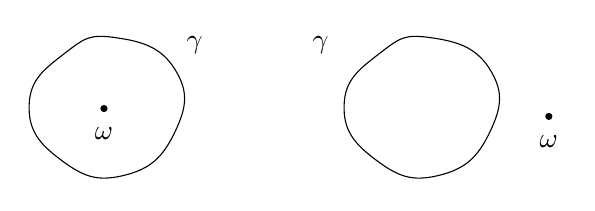
\begin{tikzpicture}[scale=1.0]
	\begin{scope}
		\draw plot[smooth cycle,tension=0.85]
			coordinates {(0.2,0.8) (0.95,0.4) (0.95,-0.4) (0.3,-0.95) (-0.5,-0.75) (-0.9,-0.05) (-0.45,0.6)};
		\node at (1.2,0.7) {$\gamma$};
		\fill (0.05,-0.1) circle (1.3pt);
		\node at (0.05,-0.42) {$\omega$};
	\end{scope}
	\begin{scope}[xshift=4cm]
		\draw plot[smooth cycle,tension=0.85]
			coordinates {(0.2,0.8) (0.95,0.4) (0.95,-0.4) (0.3,-0.95) (-0.5,-0.75) (-0.9,-0.05) (-0.45,0.6)};
		\node at (-1.2,0.7) {$\gamma$};
		\fill (1.7,-0.2) circle (1.3pt);
		\node at (1.7,-0.52) {$\omega$};
	\end{scope}
\end{tikzpicture}
\end{center}

\section{Decomposition of the spectrum}

Suppose $T : X \to X$ is bounded and $\sigma_1 \subset \sigma(T)$ is closed.

\begin{defn}
	Define $P_{\sigma_1} : X \to X$ by
	\begin{equation*}
		P_{\sigma_1} = -\frac{1}{2\pi i} \int_\Gamma \underbrace{R(z)}_{\text{resolvent}} \, dz = -\frac{1}{2\pi i} \int_\Gamma (T-z)^{-1} \, dz,
	\end{equation*}
	where $\Gamma$ is a curve enclosing only $\sigma_1$.
\end{defn}

\begin{rmk}
	This definition is independent of $\Gamma$ as long as $\Gamma$ encloses only $\sigma_1$.
\end{rmk}

\begin{rmk}
	$P_{\sigma_1}$ is bounded on $X$, since it is a Riemann integral of bounded operators.
\end{rmk}

\begin{lma}
	$P_{\sigma_1}$ is a projection.
\end{lma}
\begin{proof}
	\begin{align*}
		P_{\sigma_1}^2 &= \left( \frac{1}{2\pi i} \right)^2 \left( \int_{\Gamma_1} R(z) \, dz \right) \left( \int_{\Gamma_2} R(\omega) \, d\omega \right) \\
		&= \left( \frac{1}{2\pi i} \right)^2 \left( \iint_{\Gamma_1 \Gamma_2} R(z) R(\omega) \, d\omega \, dz \right) \\
		&= \left( \frac{-1}{2\pi i} \right)^2 \left( \iint_{\Gamma_1 \Gamma_2} \frac{R(z)}{z - \omega} \, d\omega \, dz - \iint_{\Gamma_1 \Gamma_2} \frac{R(\omega)}{z-\omega} \, d\omega \, dz \right) \\
		&= P_{\sigma_1} \quad \text{(by the calculations below).}
	\end{align*}
	Here $\Gamma_1$ is the inner curve and $\Gamma_2$ the outer curve, both enclosing $\sigma_1$:
	\begin{center}
	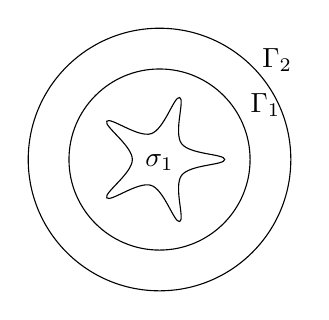
\begin{tikzpicture}[scale=1.15]
		\draw (0,0) circle (1.45);
		\node at (1.3,1.1) {$\Gamma_2$};
		\draw (0,0) circle (1.0);
		\node at (1.17,0.60) {$\Gamma_1$};
		\draw plot[smooth cycle,tension=0.65] coordinates
			{(0:0.72) (36:0.3) (72:0.72) (108:0.3) (144:0.72) (180:0.3) (216:0.72) (252:0.3) (288:0.72) (324:0.3)};
		\node at (0,-0.03) {$\sigma_1$};
	\end{tikzpicture}
	\end{center}
	\begin{align*}
		\iint_{\Gamma_1 \Gamma_2} \frac{R(z)}{z-\omega} \, d\omega \, dz &= \int_{\Gamma_1} \left( R(z) \int_{\Gamma_2} \frac{d\omega}{z - \omega} \right) dz = -2\pi i \int_{\Gamma_1} R(z) \, dz, \\
		\iint_{\Gamma_1 \Gamma_2} \frac{R(\omega)}{z-\omega} \, d\omega \, dz &= \int_{\Gamma_2} \int_{\Gamma_1} \frac{R(\omega)}{z-\omega} \, dz \, d\omega = \int_{\Gamma_2} \left( R(\omega) \underbrace{\int_{\Gamma_1} \frac{dz}{z-\omega}}_{=0} \right) d\omega = 0. \qquad\qedhere
	\end{align*}
\end{proof}

\begin{thm}
	Suppose $\sigma(T) = \sigma_1 \sqcup \sigma_2$, with $\sigma_1$ closed and nonempty and $\sigma_2$ closed.
	Then the subspaces $M = \Im P_{\sigma_1}$, $L = \ker P_{\sigma_1}$ are invariant under $T$ (i.e.\ $T(M) \subset M$, $T(L) \subset L$).
	Furthermore, $\sigma(T|_M) = \sigma_1$ and $\sigma(T|_L) = \sigma(T) \setminus \sigma_1 = \sigma_2$, with
	\begin{equation*}
		X = M \oplus L, \qquad T = \begin{bmatrix} T|_M & 0 \\ 0 & T|_L \end{bmatrix}.
	\end{equation*}
\end{thm}
\begin{proof}
	$P_{\sigma_1}$ is a bounded projection, so $X = M \oplus L$.

	\textbf{Claim: } $M$ is invariant under $T$.
	Note $T(T-z) = (T-z)T$, so $(T-z)^{-1} T = T (T-z)^{-1}$.
	Note also $T \left( \int_\Gamma R(z) \, dz \right) = \left( \int_\Gamma R(z) \, dz \right) T$ by density.
	So $T P_{\sigma_1} = P_{\sigma_1} T$.
	If $x \in M$, then $x = P_{\sigma_1} y$, and $Tx = P_{\sigma_1}(Ty) \in M$.
	Similarly, $T$ preserves $L$.

	If $\mu \notin \sigma_1$, since $\sigma_1$ is closed, there exists a curve $\gamma$ separating $\mu$ and $\sigma_1$.
	Define $S = -\frac{1}{2\pi i} \int_\gamma \frac{(T-z)^{-1}}{z - \mu} \, dz$.
	Then
	\begin{align*}
		(T-\mu)S &= -\frac{1}{2\pi i} \int_\gamma \frac{(T-\mu)(T-z)^{-1}}{z-\mu} \, dz = -\frac{1}{2\pi i} \int_\gamma \frac{(T - z + z - \mu)(T-z)^{-1}}{z - \mu} \, dz \\
		&= -\frac{1}{2\pi i} \left( \underbrace{\int_\gamma \frac{dz}{z-\mu}}_{=0} + \int_\gamma (T-z)^{-1} \, dz \right) \\
		&= P_{\sigma_1}.
	\end{align*}
	Therefore $T - \mu$ is invertible in $M$, and therefore $(T-\mu)^{-1}$ is also bounded by the open mapping theorem.
	Therefore $\mu \notin \sigma(T|_M)$.
	In other words, $\sigma(T|_M) \subseteq \sigma_1$.
	Likewise, $\sigma(T|_L) \subseteq \sigma_2$.
	Note that if $\mu \notin \sigma(T|_M) \cup \sigma(T|_L)$, then $\mu \in \rho(T)$, so
	\begin{equation*}
		\sigma(T) \subseteq \sigma(T|_M) \cup \sigma(T|_L) \subseteq \sigma_1 \sqcup \sigma_2 = \sigma(T). \qedhere
	\end{equation*}
\end{proof}

\begin{cor}
	If $\sigma_1$ is the entire spectrum, then $P_{\sigma_1} = \Id : X \to X$.
\end{cor}
\begin{proof}
	$X = M \oplus L$ and $\sigma(T|_L) = \emptyset \implies L = \lbrace 0 \rbrace$.
\end{proof}

\begin{cor}
	If $\sigma(T) = \sigma_1 \sqcup \sigma_2$, then $X = \Im(P_{\sigma_1}) \oplus \Im(P_{\sigma_2})$, and these are $T$-invariant.
	Also, $P_{\sigma_1} + P_{\sigma_2} = 1$ and $P_{\sigma_1} P_{\sigma_2} = 0$.
\end{cor}
\begin{proof}
	With $\gamma$ enclosing both $\sigma_1$ and $\sigma_2$, and $\gamma_1, \gamma_2$ enclosing $\sigma_1, \sigma_2$ respectively,
	\begin{center}
	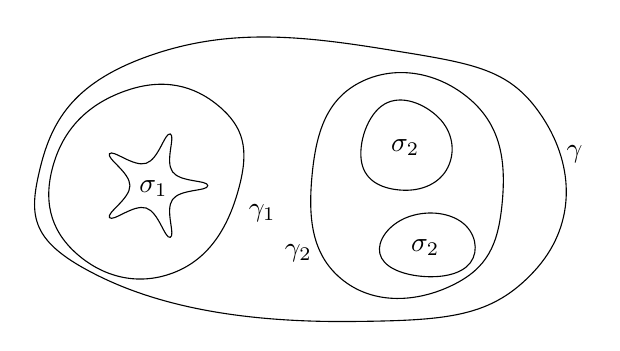
\begin{tikzpicture}[scale=1.15]
		\draw plot[smooth cycle,tension=0.8]
			coordinates {(0,1.45) (2.6,1.5) (4.3,0.75) (4.2,-0.95) (2.2,-1.5) (-0.6,-1.0) (-1.25,0.2)};
		\node at (4.65,0.35) {$\gamma$};
		\draw plot[smooth cycle,tension=0.8]
			coordinates {(-0.3,1.05) (0.72,0.88) (0.95,0.0) (0.25,-0.95) (-0.85,-0.75) (-1.1,0.25)};
		\node at (1.2,-0.3) {$\gamma_1$};
		\draw plot[smooth cycle,tension=0.75] coordinates
			{(0:0.60) (36:0.26) (72:0.60) (108:0.26) (144:0.60) (180:0.26) (216:0.60) (252:0.26) (288:0.60) (324:0.26)};
		\node at (0,-0.03) {$\sigma_1$};
		\draw plot[smooth cycle,tension=0.8]
			coordinates {(2.3,1.15) (3.5,0.95) (3.85,-0.2) (3.3,-1.1) (2.1,-1.05) (1.75,0.1)};
		\node at (1.6,-0.75) {$\gamma_2$};
		\draw plot[smooth cycle,tension=0.8]
			coordinates {(2.55,0.9) (3.15,0.75) (3.25,0.2) (2.75,-0.05) (2.3,0.25)};
		\node at (2.78,0.42) {$\sigma_2$};
		\draw plot[smooth cycle,tension=0.8]
			coordinates {(2.8,-0.35) (3.4,-0.4) (3.5,-0.85) (2.95,-1.0) (2.5,-0.75)};
		\node at (3.0,-0.68) {$\sigma_2$};
	\end{tikzpicture}
	\end{center}
	\begin{equation*}
		\int_\gamma R(z) \, dz = \int_{\gamma_1} R(z) \, dz + \int_{\gamma_2} R(z) \, dz. \qedhere
	\end{equation*}
\end{proof}

\begin{opqn}
	Is there an invariant subspace for any $T : \ell^2 \to \ell^2$?
\end{opqn}

\section{Functional calculus}

Let $T \in \cB(X)$ and take $\sigma_1 = \sigma(T)$.
Then $\Id = -\frac{1}{2\pi i} \int_\Gamma (T-z)^{-1} \, dz$, so $T = -\frac{1}{2\pi i} \int_\Gamma T(T-z)^{-1} \, dz$.
Since
\begin{equation*}
	T(T-z)^{-1} = (T - z + z)(T-z)^{-1} = \Id + z(T-z)^{-1},
\end{equation*}
we have
\begin{equation*}
	T = -\frac{1}{2\pi i} \left( \underbrace{\int_\Gamma \Id \, dz}_{=0} + \int_\Gamma z (T-z)^{-1} \, dz \right) = -\frac{1}{2\pi i} \int_\Gamma z (T-z)^{-1} \, dz.
\end{equation*}
Therefore
\begin{equation*}
	T^2 = -\frac{1}{2\pi i} \int_\Gamma z T (T-z)^{-1} \, dz = -\frac{1}{2\pi i} \int_\Gamma z \left( \Id + z(T-z)^{-1} \right) dz = -\frac{1}{2\pi i} \int_\Gamma z^2 (T-z)^{-1} \, dz,
\end{equation*}
and in general
\begin{equation*}
	T^n = -\frac{1}{2\pi i} \int_\Gamma z^n R(z) \, dz.
\end{equation*}

\begin{defn}
	Given an analytic function $f : U \subset \C \to \C$, with $U \supset \sigma(T)$, we define
	\begin{equation*}
		f(T) := -\frac{1}{2\pi i} \int_\Gamma f(z) R(z) \, dz \in \cB(X).
	\end{equation*}
\end{defn}

\begin{ex}
	Consider the problem
	\begin{equation*}
		\begin{cases}
			y'(t) = A y(t) \\
			y(0) = y_0
		\end{cases}
	\end{equation*}
	where $y : [a,b] \to X$, $A \in \cB(X)$, $y_0 \in X$.
	Solution: $y(t) = e^{tA} y_0$.
\end{ex}

\begin{ex}
	Solve equations of Sylvester type: $AZ - ZB = C$.
\end{ex}

\section{Hilbert spaces}

\begin{defn}
	A Banach space $X$ whose norm comes from an inner product, i.e.\ $\norm{u}^2 = \ip{u}{u}$ with $\ip{\cdot}{\cdot} : X \times X \to \C$ bilinear, is called a \underline{Hilbert space}.
\end{defn}

\begin{thm}[Parallelogram identity]
	If $X$ is Hilbert, then
	\begin{equation*}
		\norm{u+v}^2 + \norm{u-v}^2 = 2 \left( \norm{u}^2 + \norm{v}^2 \right). \tag{P}
	\end{equation*}
	Conversely, if a norm satisfies (P), then it comes from an inner product.
\end{thm}
\begin{proof}
	$\norm{u+v}^2 = \ip{u+v}{u+v} = \norm{u}^2 + 2\ip{u}{v} + \norm{v}^2$, so
	\begin{equation*}
		\norm{u+v}^2 + \norm{u-v}^2 = 2 \left( \norm{u}^2 + \norm{v}^2 \right).
	\end{equation*}
	For the converse, set $\ip{u}{v} := \frac{\norm{u+v}^2 - \norm{u}^2 - \norm{v}^2}{2}$.
\end{proof}

\begin{ex}
	$\ell^p$ is Hilbert iff $p = 2$, with $\ip{u}{v} = \sum_{i=1}^\infty u_i \bar{v}_i$.
	Indeed,
	\begin{equation*}
		\norm{e_1 + e_2}_p^2 + \norm{e_1 - e_2}_p^2 = 2^{2/p} + 2^{2/p}, \qquad 2 \left( \norm{e_1}^2 + \norm{e_2}^2 \right) = 4,
	\end{equation*}
	so $2^{2/p} = 2 \implies p = 2$.
\end{ex}

\begin{ex}
	$L^p$ is Hilbert $\iff p = 2$, with $\ip{f}{g}_{L^2} = \int_\R f(x) \overline{g(x)} \, dx$.
\end{ex}

\begin{lma}
	If $H$ is Hilbert, with $\norm{u}^2 = \ip{u}{u}$, then $\ip{\cdot}{\cdot} : H \times H \to \R$ is continuous.
\end{lma}
\begin{proof}
	Cauchy--Schwarz: $\abs{\ip{u}{v}} \leq \norm{u} \cdot \norm{v}$.
\end{proof}

\begin{rmk}
	For a multilinear map $T : \underbrace{X \times X \times \cdots \times X}_{N} \to Y$, being continuous is equivalent to being bounded, where
	\begin{equation*}
		\norm{T(x_1, x_2, \dots, x_N)}_Y \leq C \norm{x_1}_X \cdots \norm{x_N}_X.
	\end{equation*}
\end{rmk}

\section{Orthogonal complements and projections}

\begin{defn}
	Let $H$ be a Hilbert space and $M$ a subspace.
	Then we can write
	\begin{equation*}
		M^\perp := \lbrace x \in H : \ip{x}{m} = 0 \ \forall m \in M \rbrace,
	\end{equation*}
	the \underline{orthogonal complement}.
\end{defn}

\begin{fct}
	$(M^\perp)^\perp = \overline{M}$.
\end{fct}

\begin{rmk}
	It is not always true that $H = M \oplus M^\perp$.
\end{rmk}

\begin{ex}
	If $M$ is dense but $M \neq H$, then if $y \in M^\perp$, $\ip{m}{y} = 0$ for all $m \in M$.
	But there exists $\lbrace y_n \rbrace \to y$ with $\lbrace y_n \rbrace \subseteq M$, so
	\begin{equation*}
		0 = \ip{y_n}{y} \to \ip{y}{y} = \norm{y}^2.
	\end{equation*}
\end{ex}

\begin{lma}
	Let $C$ be a nonempty closed convex subset of $H$.
	Then there exists a unique element $h_0 \in C$ which minimizes the norm: $\norm{h_0} = \inf \lbrace \norm{h} : h \in C \rbrace$.
\end{lma}
\begin{proof}
	Consider the parallelogram identity
	\begin{equation*}
		\norm{\frac{x-y}{2}}^2 = \tfrac{1}{2} \left( \norm{x}^2 + \norm{y}^2 \right) - \norm{\frac{x+y}{2}}^2.
	\end{equation*}
	Take a sequence $\lbrace x_n \rbrace$ in $C$ such that $\norm{x_n} \to \alpha$.

	\textbf{Claim: } $\lbrace x_n \rbrace$ is Cauchy.
	\begin{equation*}
		0 \leq \norm{\frac{x_n - x_m}{2}}^2 = \tfrac{1}{2} \left( \norm{x_n}^2 + \norm{x_m}^2 \right) - \norm{\underbrace{\frac{x_n + x_m}{2}}_{\in C}}^2 \leq \underbrace{\tfrac{1}{2} \left( \norm{x_n}^2 + \norm{x_m}^2 \right) - \alpha^2}_{\to 0}.
	\end{equation*}
	Therefore $(x_n)$ converges to $x \in C$ since $C$ is closed, and $\norm{x} = \alpha$.
	If $y \in C$ with $\norm{y} = \alpha$, then
	\begin{equation*}
		\norm{\frac{x-y}{2}}^2 = \alpha^2 - \norm{\frac{x}{2} + \frac{y}{2}}^2 \leq \alpha^2 - \alpha^2 = 0. \qedhere
	\end{equation*}
\end{proof}

\begin{cor}
	If $C$ is a nonempty closed convex set in $H$ and $x \in H$, then there exists a unique distance minimizer: $d(x,C) = d(x,h_0)$, $h_0 \in C$.
\end{cor}

\begin{thm}
	Let $H$ be Hilbert and $M \subseteq H$ a closed subspace.
	Then there exist projections $P : H \to M$, $Q : H \to M^\perp$ such that
	\begin{enumerate}[label=(\roman*),nosep]
		\item $\forall x \in H$, $x = Px + Qx$;
		\item $Px$ is the closest point to $x$ in $M$, and $Qx$ the closest in $M^\perp$;
		\item $P, Q \in \cB(H)$;
		\item $\norm{x}^2 = \norm{Px}^2 + \norm{Qx}^2$ for all $x$;
		\item $P, Q$ are the unique projections with these properties.
	\end{enumerate}
\end{thm}
\begin{proof}
	Define $P(x) = $ the closest point to $x$ in $M$, and define $Q(x) = x - Px$.
	We get (i) for free.

	\textbf{Claim: } $Qx \in M^\perp$.
	Let $m \in M$.
	Assume WLOG $\norm{m} = 1$.
	Let $t \in \R$.
	Then
	\begin{align*}
		\norm{Qx - tm}^2 = \norm{x - Px - tm}^2 &\geq \norm{x - Px}^2 \\
		\norm{x-Px}^2 - 2t\ip{x-Px}{m} + t^2 \norm{m}^2 &\geq \norm{x-Px}^2 \\
		-2t \ip{Qx}{m} + t^2 &\geq 0.
	\end{align*}
	Let $t = \ip{Qx}{m}$:
	\begin{align*}
		-2\ip{Qx}{m}^2 + \ip{Qx}{m}^2 &\geq 0 \\
		\implies 0 \geq -\ip{Qx}{m}^2 &\geq 0 \\
		\implies \ip{Qx}{m} &= 0.
	\end{align*}

	\textbf{Claim: } $Qx$ is the closest point to $x$ in $M^\perp$.
	Let $y \in M^\perp$.
	Then $\norm{x-y}^2 = \norm{Px}^2 + \norm{Qx-y}^2$.
	The only way to minimize the right-hand side is $\norm{Qx - y}^2 = 0$.

	\textbf{Claim: } $P$ and $Q$ are linear.
	\begin{align*}
		x + y &= P(x+y) + Q(x+y) \\
		x + y &= (P(x) + Q(x)) + (P(y) + Q(y)) \\
		\underbrace{P(x+y) - P(x) - P(y)}_{\in M} &= -\underbrace{\left( Q(x+y) - Q(x) - Q(y) \right)}_{\in M^\perp}.
	\end{align*}

	(iv) $\norm{x}^2 = \ip{Px + Qx}{Px + Qx} = \norm{Px}^2 + \norm{Qx}^2$.
	In particular, $\norm{Px}^2 \leq \norm{x}^2$, so $\norm{P}_{\mathrm{op}} \leq 1$, with $\norm{P}_{\mathrm{op}} = 1$ if $M \neq \lbrace 0 \rbrace$.

	(v) If $P', Q'$ are another pair of projections, then
	\begin{align*}
		x = Px + Qx &= P'x + Q'x \\
		\implies -(Px - P'x) &= Qx - Q'x \\
		\implies Px - P'x &\in M \cap M^\perp \\
		\implies Px &= P'x. \qedhere
	\end{align*}
\end{proof}

\section{The Riesz representation theorem}

\begin{thm}[Riesz Representation]
	Let $H$ be a Hilbert space and $\varphi \in H^*$.
	Then there exists a unique $z \in H$ such that $\varphi(x) = \ip{x}{z}$ for all $x$.
	Furthermore, $\norm{\varphi}_{\mathrm{op}} = \norm{z}$.
\end{thm}
\begin{proof}
	If $\varphi = 0$, then $z = 0$.
	If not, let $M = \ker \varphi$.
	Then $M$ is closed and $H = M \oplus M^\perp$.
	Choose $y \in M^\perp$ such that $\varphi(y) = 1$.
	Now given $x \in H$, note that $x - \varphi(x) y \in M = \ker \varphi$.
	For all $x$, $x - \varphi(x)y \perp y \iff \ip{x - \varphi(x)y}{y} = 0$, so
	\begin{equation*}
		\ip{x}{y} - \varphi(x) \ip{y}{y} = 0 \implies \varphi(x) = \ip{x}{\frac{y}{\norm{y}^2}},
	\end{equation*}
	so let $z = \frac{y}{\norm{y}^2}$.
	Then
	\begin{equation*}
		\abs{\varphi(x)} = \abs{\ip{x}{z}} \leq \norm{x} \cdot \norm{z} \implies \forall x \neq 0, \ \abs{\varphi\left( \tfrac{x}{\norm{x}} \right)} \leq \norm{z} \implies \norm{\varphi}_{\mathrm{op}} \leq \norm{z},
	\end{equation*}
	and
	\begin{equation*}
		\abs{\varphi\left( \tfrac{z}{\norm{z}} \right)} = \frac{\norm{z}^2}{\norm{z}} = \norm{z},
	\end{equation*}
	so $\norm{\varphi}_{\mathrm{op}} = \norm{z}$.

	Uniqueness: $\ip{x}{z} = \ip{x}{z'}$ for all $x$ $\implies \ip{x}{z - z'} = 0$ for all $x$ $\implies z - z' = 0$.
\end{proof}

\begin{cor}
	$H^* \cong H$.
\end{cor}

\section{Orthonormal bases}

\begin{defn}
	A subset $E \subset H$ is an \underline{orthonormal set} if for all $u, v \in E$, $\ip{u}{v}$ is $1$ if $u = v$ and $0$ otherwise.
\end{defn}

\begin{defn}
	$E \subset H$ is an \underline{orthonormal basis} if it is orthonormal and \underline{maximal} with respect to inclusion, i.e.\ $E \subsetneq E' \implies E'$ is not orthonormal.
\end{defn}

\begin{lma}[Bessel's inequality]
	If $E$ is an orthonormal set, $E = \lbrace e_j \rbrace_{j \in J}$, then
	\begin{equation*}
		\sum_j \abs{\ip{v}{e_j}}^2 \leq \norm{v}^2 \quad \forall v \in H.
	\end{equation*}
\end{lma}
\begin{proof}
	\begin{align*}
		0 \leq \norm{v - \sum_j \ip{v}{e_j} e_j}^2 &= \ip{v - \sum_j \ip{v}{e_j}e_j}{v - \sum_j \ip{v}{e_j}e_j} \\
		&= \norm{v}^2 - 2\sum_k \abs{\ip{v}{e_k}}^2 + \sum_{j,k} \ip{v}{e_j} \ip{v}{e_k} \ip{e_j}{e_k} \\
		&= \norm{v}^2 - \sum_k \abs{\ip{v}{e_k}}^2. \qedhere
	\end{align*}
\end{proof}

\begin{thm}
	Let $E = \lbrace e_j \rbrace_{j \in \N}$ be an orthonormal set.
	TFAE:
	\begin{enumerate}[label=(\roman*),nosep]
		\item $E$ is an orthonormal basis.
		\item If $v \perp E$, then $v = 0$.
		\item $\forall v \in H$, $v = \sum_j \ip{v}{e_j} e_j$.
		\item $\forall v \in H$, there exists a sequence of scalars $\alpha_j$ such that $v = \sum_j \alpha_j e_j$.
		\item $\forall v \in H$, $\norm{v}^2 = \sum_j \abs{\ip{v}{e_j}}^2$.
		\item $\forall u, v \in H$, $\ip{u}{v} = \sum_j \ip{u}{e_j} \overline{\ip{v}{e_j}}$.
	\end{enumerate}
\end{thm}
\begin{proof}
	(i $\implies$ ii) Definition.

	(ii $\implies$ i) Contrapositive.

	(ii $\implies$ iii) \textbf{Claim: } $S_n = \sum_{j=1}^n \ip{v}{e_j} e_j$ is Cauchy.
	WLOG $m > n$:
	\begin{equation*}
		\norm{S_n - S_m}^2 = \norm{\sum_{j=n+1}^m \ip{v}{e_j} e_j}^2 = \sum_{j=n+1}^m \abs{\ip{v}{e_j}}^2 \xrightarrow{n,m \to \infty} 0.
	\end{equation*}
	Let $\omega = \sum_1^\infty \ip{v}{e_j} e_j$.
	Then
	\begin{equation*}
		\ip{v - \omega}{e_{j_0}} = \ip{v}{e_{j_0}} - \sum_1^\infty \ip{v}{e_j} \ip{e_j}{e_{j_0}} = 0.
	\end{equation*}
	Thus $v - \omega$ is orthogonal to $E$, so $v - \omega = 0$.

	(iii $\implies$ ii) $v = \sum \ip{v}{e_j} e_j = 0$.

	(iv $\implies$ iii)
	\begin{equation*}
		\ip{v}{e_k} = \ip{\sum_{j=1}^\infty a_j e_j}{e_k} = \sum_{j=1}^\infty a_j \ip{e_j}{e_k} = a_k.
	\end{equation*}

	(iii $\implies$ v)
	\begin{equation*}
		\norm{\sum_{j=1}^N \ip{v}{e_j} e_j}^2 = \sum_{j=1}^N \abs{\ip{v}{e_j}}^2, \qquad \norm{v}^2 = \sum_{j=1}^\infty \abs{\ip{v}{e_j}}^2. \qedhere
	\end{equation*}
\end{proof}

\begin{rmk}
	If $S \subset H$ is spanned by an orthonormal basis $e_1, \dots, e_m$, then the orthogonal projection is
	\begin{equation*}
		P_S(v) = \sum_{j=1}^m \ip{v}{e_j} e_j.
	\end{equation*}
\end{rmk}

\section{Compact operators}

\begin{defn}
	An operator $T : X \to Y$ (Banach spaces) is \underline{compact} if for any bounded sequence $\lbrace x_n \rbrace$ in $X$, $\lbrace Tx_n \rbrace$ has a convergent subsequence.
\end{defn}

\begin{prop}
	$T$ compact $\implies T$ bounded.
\end{prop}
\begin{proof}
	Suppose not.
	There exists $\lbrace x_n \rbrace$ of unit vectors in $X$ where $\norm{Tx_n} \to \infty$.
	If $x_n \to x$, then $\norm{x_n} \to \norm{x}$, so then $\norm{Tx_n}$ has no convergent subsequence.
\end{proof}

\begin{ex}
	$T : \R^n \to \R^n$ is compact.
	Let $(x_n)$ be bounded.
	Then
	\begin{equation*}
		\norm{T(x_n)} \leq \norm{T}_{\mathrm{op}} \norm{x_n} \leq C \norm{T}_{\mathrm{op}},
	\end{equation*}
	and Heine--Borel gives that $B_{C\norm{T}_{\mathrm{op}}}(0)$ is compact, so $\lbrace Tx_n \rbrace$ has a convergent subsequence.
\end{ex}

\begin{ex}
	$R : \ell^2 \to \ell^2$, $R(x_1, x_2, \dots) = (0, x_1, x_2, \dots)$.
	Then $Re_n = e_{n+1}$ for all $n$, and $(e_n)$ is bounded, but $(Re_n)$ has no convergent subsequence.
\end{ex}

\begin{ex}
	$T : \ell^2 \to \ell^2$, $T(x_1, x_2, \dots) = (x_1, x_2, x_3, 0, 0, \dots)$.
	\begin{itemize}[nosep]
		\item $\Im T$ is finite-dimensional.
		\item $T$ is bounded.
	\end{itemize}
	Therefore $T$ is compact by a similar proof to the $T : \R^n \to \R^n$ example.
\end{ex}

\begin{ex}
	$T : \ell^2 \to \ell^2$, $(x_1, x_2, \dots) \mapsto \left( x_1, \frac{x_2}{2}, \frac{x_3}{3}, \frac{x_4}{4}, \dots \right)$ is compact, because it is the limit of a sequence of finite rank operators:
	\begin{align*}
		T_1 &: (x_1, x_2, \dots) \mapsto (x_1, 0, 0, \dots) \\
		T_2 &: (x_1, x_2, \dots) \mapsto \left( x_1, \tfrac{x_2}{2}, 0, 0, \dots \right).
	\end{align*}
	Then
	\begin{equation*}
		\norm{(T - T_n)x}^2 = \norm{\left( 0, 0, \dots, 0, \tfrac{x_{n+1}}{n+1}, \dots \right)}^2 = \sum_{j=n+1}^\infty \frac{x_j^2}{j^2} \leq \frac{1}{(n+1)^2} \quad \text{for } \norm{x} = 1,
	\end{equation*}
	so $\norm{T - T_n}_{\mathrm{op}} \leq \frac{1}{n+1} \to 0$.
\end{ex}

\begin{thm}
	$T : \ell^2 \to \ell^2$, $T(x_1, x_2, \dots) = (a_1x_1, a_2x_2, \dots)$ is compact iff $\lim_n a_n = 0$.
\end{thm}

\begin{rmk}
	$c_0 \cong$ diagonal, compact operators in $\ell^2$, and $\ell^p \hookrightarrow$ diagonal, compact operators in $\ell^2$:
	\begin{align*}
		\varphi : \ell^p &\to \cB(\ell^2) \\
		\lbrace a_n \rbrace &\mapsto D_{\lbrace a_n \rbrace} : \ell^2 \to \ell^2 \\
		&\qquad\qquad\ (x_n) \mapsto (a_n x_n).
	\end{align*}
	Then $\varphi(\ell^p) \subset \cB(\ell^2)$ is called the \underline{Schatten $p$-class}.
	\begin{itemize}[nosep]
		\item For $p=1$: these are called \underline{trace-class} operators.
		\item For $p=2$: these are \underline{Hilbert--Schmidt} operators.
	\end{itemize}
\end{rmk}

\begin{thm}
	Let $X$ be a Banach space and $\cK(X)$ the set of compact operators $X \to X$.
	Then:
	\begin{enumerate}[label=(\roman*),nosep]
		\item $\cK(X)$ is a subspace of $\cB(X)$.
		\item If $T \in \cK(X)$, $S \in \cB(X)$, then $TS$ and $ST$ are compact, i.e.\ $\cK(X)$ is an ideal of $\cB(X)$.
		The quotient $\cC(X) = \cB(X)/\cK(X)$ is the \underline{Calkin algebra}.
	\end{enumerate}
\end{thm}
\begin{proof}
	(i) Let $T_1, T_2 \in \cK(X)$ and let $\lbrace x_n \rbrace$ be a bounded sequence.
	$T_1(x_n)$ has a convergent subsequence, say $T_1(x_{n,1})$.
	Then $T_2(x_{n,1})$ has a convergent subsequence, say $T_2(x_{n,2})$.
	Therefore $(T_1 + T_2)(x_{n,2})$ converges.

	(ii) $(x_n)$ bounded $\implies (Sx_n)$ bounded $\implies T(Sx_n)$ has a convergent subsequence.
	$(x_n)$ bounded $\implies (Tx_n)$ has a convergent subsequence $\implies S(Tx_n)$ has a convergent subsequence.
\end{proof}

\begin{thm}
	$\cK(X) \subset \cB(X)$ is closed.
\end{thm}
\begin{proof}
	Let $\lbrace T_j \rbrace$ be a sequence in $\cK(X)$ such that $T_j \xrightarrow{\mathrm{op}} T \in \cB(X)$.
	Let $\lbrace x_n \rbrace$ be a sequence in $X$ such that $\norm{x_n} \leq M$ for all $n$.
	$T_1(x_n)$ has a convergent subsequence $(x_{n,1})$;
	$T_2(x_{n,1})$ has a convergent subsequence $(x_{n,2})$;
	and so on.
	Therefore $T_j(x_{n,k})$ converges as $n \to \infty$ for any $k \geq j$.
	Now consider $(x_{n,n})$.

	\textbf{Claim: } $\lbrace Tx_{n,n} \rbrace$ converges.
	\begin{equation*}
		\norm{Tx_{n,n} - Tx_{m,m}} \leq \norm{Tx_{n,n} - T_jx_{n,n}} + \norm{T_jx_{n,n} - T_jx_{m,m}} + \norm{T_jx_{m,m} - Tx_{m,m}}.
	\end{equation*}
	Let $\varepsilon > 0$.
	We have
	\begin{equation*}
		\norm{Tx_{n,n} - T_jx_{n,n}} \leq \norm{T - T_j}_{\mathrm{op}} \cdot M, \qquad \norm{T_jx_{m,m} - Tx_{m,m}} \leq M \norm{T-T_j}_{\mathrm{op}},
	\end{equation*}
	so
	\begin{equation*}
		\norm{Tx_{n,n} - Tx_{m,m}} \leq \underbrace{2M \norm{T-T_j}_{\mathrm{op}}}_{< \varepsilon/2} + \underbrace{\norm{T_j x_{n,n} - T_j x_{m,m}}}_{< \varepsilon/2}.
	\end{equation*}
	Pick $j$ large enough.
\end{proof}

\begin{cor}
	$T : \ell^2 \to \ell^2$, $T(x) = (a_1x_1, a_2x_2, \dots)$ is compact when $\lim_{n \to \infty} a_n = 0$.
\end{cor}

\begin{qn}
	Is every compact operator $T \in \cK(X)$, $X$ Banach separable, the limit of finite rank operators?
	That is, is $\overline{\Fin(X)} = \cK(X)$?
\end{qn}

\noindent Per Enflo: no! (1973) (He was rewarded with a live goose.)

\begin{thm}
	If $H$ is Hilbert, then the question is true: $\overline{\Fin(H)} = \cK(H)$.
\end{thm}
\begin{proof}
	Prove for $H$ separable.
	Let $T : H \to H$ be compact.
	Let $V = \overline{\Im T}$.
	Let $(e_n)$ be an orthonormal basis of $V$.
	Define
	\begin{equation*}
		T_n(h) = \sum_1^n \ip{Th}{e_j} e_j = P_n(Th),
	\end{equation*}
	where $P_n$ projects onto $\spn(e_1, \dots, e_n)$.

	\textbf{Claim: } $T_n h \to Th$ as $n \to \infty$, because basis.
	Since $T$ is compact, $\overline{T(B_1(0))}$ is compact.
	Given $\varepsilon > 0$, there exist a finite number of vectors $h_1, \dots, h_N \in B_1(0)$ such that $\overline{T(B_1(0))} \subset \bigcup B_\varepsilon(Th_j)$.
	For any $h \in B_1(0)$ we have
	\begin{equation*}
		\norm{T_n h - Th} \leq \norm{T_n h - T_n h_j} + \norm{T_n h_j - Th_j} + \underbrace{\norm{Th_j - Th}}_{< \varepsilon},
	\end{equation*}
	where
	\begin{equation*}
		\norm{T_nh - T_nh_j} = \norm{P_nT(h) - P_n(T(h_j))} \leq \underbrace{\norm{T(h) - T(h_j)}}_{< \varepsilon}.
	\end{equation*}
	Convergence then gives $\norm{T_nh_j - Th_j} \xrightarrow{n \to \infty} 0$.
	Therefore $\norm{T_n - T}_{\mathrm{op}} \to 0$.
\end{proof}

\section{The Fredholm alternative}

\begin{thm}[Fredholm Alternative]
	Let $T \in \cK(X)$.
	Then $\sigma(T) \setminus \lbrace 0 \rbrace \subseteq \sigma_p(T)$.
	Alternatively, for any $\lambda \neq 0$, one of the following holds:
	\begin{enumerate}[nosep]
		\item The equation $Tx = \lambda x$ has a nonzero solution $x$.
		\item $(T-\lambda) : X \to X$ is invertible, i.e.\ the equation $(T-\lambda)x = y$ has a unique solution $x$ for any $y$.
	\end{enumerate}
\end{thm}

\begin{lma}
	If $T \in \cK(X)$, $\lambda \neq 0$, $\lambda \notin \sigma_p(T)$, we have a lower bound
	\begin{equation*}
		\exists c : \norm{(T-\lambda)x} \geq c\norm{x} \quad \forall x.
	\end{equation*}
\end{lma}
\begin{proof}
	Suppose not.
	Then there exists a sequence of unit vectors $(x_n)$ such that $(T-\lambda)x_n \to 0$.
	By compactness of $T$, $Tx_n \to y$.
	Note $y \neq 0$.
	Then
	\begin{equation*}
		T(\underbrace{(T-\lambda)x_n}_{T(0) = 0}) = (T-\lambda)Tx_n \to (T-\lambda)y,
	\end{equation*}
	so $(T-\lambda)y = 0$, and therefore $\lambda \in \sigma_p(T)$, a contradiction.
\end{proof}

\begin{lma}
	$\Im(T-\lambda)$ is a closed subspace of $H$, for $\lambda \notin \sigma_p(T)$.
\end{lma}
\begin{proof}
	We can rewrite the previous equation as $\norm{x} \leq \frac{1}{c} \norm{(T-\lambda)x}$ for all $x$.
	Suppose $\underbrace{(T-\lambda)x_n}_{z_n} \to z$.
	Then
	\begin{equation*}
		\norm{x_n - x_m} \leq \tfrac{1}{c} \norm{(T-\lambda)x_n - (T-\lambda)x_m} = \tfrac{1}{c} \norm{z_n - z_m} \to 0.
	\end{equation*}
	Therefore it is Cauchy, so $x_n \to x$, and $(T-\lambda)x_n \to (T-\lambda)x \in \Im(T-\lambda)$.
\end{proof}

\begin{proof}[Proof of the theorem]
	Assume (1) does not hold.
	Let $V = \Im(T-\lambda)$.
	We have $T - \lambda : H \to V$.
	Assume $V \neq H$.
	Define the following sequence: $V_n := \Im(T-\lambda)^n$, $n = 1, 2, 3, \dots$, so $V_1 = V$.

	\textbf{Claim: } $V_1 \supset V_2 \supset V_3 \supset \cdots$, every inclusion proper.
	If not, then for all $y \in H$ there exists $x \in V_2$ such that $(T-\lambda)y = (T-\lambda)^2x$.
	But then $y = (T-\lambda)x$, contradicting $V \neq H$.

	Pick $x_n \in V_n$ such that $d(x_n, V_{n+1}) = \frac{1}{2}$ for all $n$.
	Then
	\begin{align*}
		\norm{Tx_1 - Tx_2} = \norm{Tx_1 - \lambda x_1 + \lambda x_1 - Tx_2} &= \norm{\lambda x_1 + \underbrace{(T-\lambda)x_1}_{\in V_2} - \underbrace{Tx_2}_{\in V_2}} \\
		&= \abs{\lambda} \norm{x_1 - \underbrace{\omega}_{\in V_2}} \geq \abs{\lambda} \cdot \tfrac{1}{2}.
	\end{align*}
	Therefore $\norm{Tx_1 - Tx_2} \geq \frac{\abs{\lambda}}{2}$.
	More generally, $\norm{Tx_n - Tx_m} \geq \frac{\abs{\lambda}}{2}$ for $n \neq m$.
\end{proof}

\section{Adjoints}

Let $H$ be a Hilbert space and $T \in \cB(H)$.

\begin{defn}
	Given $y \in H$, define $\varphi : H \to \C$ by $\varphi(x) = \ip{Tx}{y}$.
\end{defn}

\begin{rmk}
	$\abs{\varphi(x)} = \abs{\ip{Tx}{y}} \leq \norm{Tx} \cdot \norm{y} \leq \norm{T}_{\mathrm{op}} \norm{x} \cdot \norm{y} \leq M \norm{x}$, so $\varphi$ is bounded linear.
	By Riesz representation, there exists a unique vector $T^*y$ such that
	\begin{equation*}
		\ip{Tx}{y} = \ip{x}{T^*y} \quad \forall x, \forall y.
	\end{equation*}
	We call $y \mapsto T^*y$ the \underline{adjoint} of $T$.
\end{rmk}

\begin{ex}
	$T : \C^n \to \C^n$, with $\lbrace e_1, \dots, e_n \rbrace$ the standard basis.
	The matrix of $T$ is given by $T_{ij} = \ip{Te_i}{e_j}$.
	The matrix of $T^*$ is given by
	\begin{equation*}
		(T^*)_{ji} = \ip{T^*e_i}{e_j} = \overline{\ip{e_i}{Te_j}} = \overline{\ip{Te_j}{e_i}} = \overline{T_{ji}}.
	\end{equation*}
	Recall: on $\C^n$, the inner product is $\ip{z}{\omega} = \sum_{i=1}^n z_i \bar{\omega}_i$.
\end{ex}

\begin{ex}
	Recall $R : \ell^2 \to \ell^2$, $R(x_1, x_2, \dots) = (0, x_1, x_2, \dots)$.
	\textbf{Q: } What is $R^*$?
	Answer: $R^* = L$, since
	\begin{equation*}
		\ip{R^*e_m}{e_k} = \ip{e_m}{Re_k} = \ip{e_m}{e_{k+1}} = \delta_{m,k+1}.
	\end{equation*}
\end{ex}

\begin{ex}
	Let $\varphi : [0,1] \to \C$ be continuous.
	Consider $M_\varphi : L^2[0,1] \to L^2[0,1]$, $f \mapsto \varphi f$.
	Then $M_\varphi^* = M_{\bar\varphi}$, since
	\begin{equation*}
		\ip{M_\varphi f}{g}_{L^2} = \int_0^1 \varphi f \bar{g} \, dx = \int_0^1 f \cdot \overline{(\bar\varphi g)} \, dx = \ip{f}{M_{\bar\varphi} g}_{L^2}.
	\end{equation*}
	If $\varphi$ is real ($\varphi : [0,1] \to \R$), then $M_\varphi^* = M_\varphi$ (\underline{self-adjoint}).
\end{ex}

\begin{rmk}
	Recall that $(M f)(t) = t f(t)$ has no eigenvalues but is self-adjoint.
\end{rmk}

\begin{thm}
	\begin{enumerate}[label=(\roman*),nosep]
		\item $T^* \in \cB(H)$.
		\item $\norm{T^*}_{\mathrm{op}} = \norm{T}_{\mathrm{op}}$.
		\item $(\alpha T + S)^* = \bar{\alpha} T^* + S^*$ for all $T, S \in \cB(H)$.
		\item $(TS)^* = S^*T^*$.
	\end{enumerate}
\end{thm}
\begin{proof}
	(i) $T^*$ is linear: let $y_1, y_2 \in H$, $\alpha \in \C$.
	Then for any $x \in H$,
	\begin{align*}
		\ip{Tx}{\alpha y_1 + y_2} &= \ip{x}{T^*(\alpha y_1 + y_2)} \\
		\bar{\alpha} \ip{Tx}{y_1} + \ip{Tx}{y_2} &= \bar{\alpha}\ip{x}{T^*y_1} + \ip{x}{T^*y_2} = \ip{x}{\alpha T^*y_1 + T^*y_2}.
	\end{align*}
	By Riesz representation,
	\begin{equation*}
		\norm{T^*y} = \norm{\ip{T(\cdot)}{y}}_{\mathrm{op}} = \sup_{\norm{x}=1} \abs{\ip{Tx}{y}} \leq \norm{T} \cdot \norm{y} \quad \forall y.
	\end{equation*}
	Therefore $\norm{T^*}_{\mathrm{op}} \leq \norm{T}_{\mathrm{op}}$ and $\underbrace{\norm{T^{**}}_{\mathrm{op}}}_{= \norm{T}_{\mathrm{op}}} \leq \norm{T^*}_{\mathrm{op}}$.
\end{proof}

\section{Kernel--image duality}

\begin{rmk}
	If $S \subset H$, then $(S^\perp)^\perp = \overline{S}$.
\end{rmk}

\begin{thm}[Kernel--Image Duality]
	Let $T : H \to H$ be bounded.
	Then $\ker(T) = (\Im(T^*))^\perp$.
\end{thm}
\begin{proof}
	\begin{equation*}
		(x \in \ker T) \iff (\ip{Tx}{y} = 0 \ \forall y) \iff (\ip{x}{T^*y} = 0 \ \forall y) \iff (x \perp \Im T^*). \qedhere
	\end{equation*}
\end{proof}

\begin{cor}
	\begin{align*}
		\ker(T^*) &= \Im(T)^\perp \\
		\ker(T)^\perp &= \overline{\Im(T^*)} \\
		\ker(T^*)^\perp &= \overline{\Im(T)}
	\end{align*}
\end{cor}

\begin{thm}
	$T$ compact $\implies T^*$ compact.
\end{thm}
\begin{proof}[Proof 1]
	Let $T$ be compact.
	Then
	\begin{equation*}
		\norm{T^*v}^2 = \abs{\ip{T^*v}{T^*v}} = \abs{\ip{TT^*v}{v}} \leq \norm{TT^*v} \cdot \norm{v}. \tag{1}
	\end{equation*}
	Let $v_n$ be a bounded sequence.
	Then
	\begin{equation*}
		\norm{T^*v_n - T^*v_m}^2 \leq \norm{TT^*v_n - TT^*v_m} \cdot \norm{v_n - v_m} \leq 2M \norm{TT^*v_n - TT^*v_m}.
	\end{equation*}
	By compactness of $TT^*$, there exists a convergent subsequence $TT^*v_{n_k}$.
	Therefore by (1), $T^*v_{n_k}$ converges.
\end{proof}
\begin{proof}[Proof 2]
	Let $\varepsilon > 0$.
	There exists $F \in \Fin(H)$ such that $\norm{T - F}_{\mathrm{op}} < \varepsilon$.
	Assuming $F^*$ is also finite rank, we get $\norm{T^* - F^*}_{\mathrm{op}} < \varepsilon$.

	\textbf{Claim: } $F^*$ has finite rank if $F$ does.
	$\Im(F)$ is finite-dimensional, and $\Im(F) = \ker(F^*)^\perp$, so $\Im(F)^\perp = \ker(F^*)$, giving
	\begin{equation*}
		H = \underbrace{\Im(F)}_{\text{fin-dim}} \oplus \underbrace{\Im(F)^\perp}_{\ker(F^*)}. \qedhere
	\end{equation*}
\end{proof}

\begin{lma}
	Let $T$ be compact and $\lambda \neq 0$.
	Then $\ker(T-\lambda)$ is finite-dimensional.
\end{lma}
\begin{proof}
	$T(\ker(T-\lambda)) \subset \ker(T-\lambda)$ because $T$ commutes with $T-\lambda$.
	For $x \in \ker(T-\lambda)$, $Tx = (T-\lambda)x + \lambda x = \lambda x$.
	So $T|_{\ker(T-\lambda)} = \lambda \cdot \Id|_{\ker(T-\lambda)}$, so $\lambda \Id$ is compact, and therefore $\dim \ker(T-\lambda) < \infty$.
\end{proof}

\begin{lma}
	If $T$ is compact and $\lambda \neq 0$, then $T - \lambda$ is \underline{bounded from below} on $(\ker(T-\lambda))^\perp$, i.e.
	\begin{equation*}
		\norm{(T-\lambda)x} \geq c \norm{x}, \quad x \in \ker(T-\lambda)^\perp.
	\end{equation*}
\end{lma}

\noindent It follows from this lemma that $\Im(T-\lambda)$ is closed.

\begin{ex}
	$T(x_1, x_2, \dots) = \left( x_1, \frac{x_2}{2}, \frac{x_3}{3}, \dots \right)$ is a good example of compact but not finite rank.
\end{ex}

\begin{thm}
	Let $T$ be compact and $\lambda \neq 0$.
	Then the equation $(T-\lambda)x = y$ is solvable iff $y \in \ker(T^* - \bar{\lambda})^\perp$.
\end{thm}
\begin{proof}
	$(T-\lambda)x = y$ solvable $\iff y \in \Im(T-\lambda) \iff y \in \ker((T-\lambda)^*)^\perp$.
\end{proof}

\begin{thm}
	Let $T$ be compact and $\lambda \neq 0$.
	Then $T - \lambda$ is injective $\iff T - \lambda$ is surjective.
\end{thm}
\begin{proof}
	$T-\lambda$ injective $\implies T-\lambda$ surjective by the Fredholm alternative.

	Conversely,
	\begin{align*}
		T - \lambda \text{ surjective} &\implies \Im(T-\lambda) = H = \ker(T^* - \bar{\lambda})^\perp \\
		&\implies T^* - \bar{\lambda} \text{ injective} \\
		&\implies T^* - \bar{\lambda} \text{ surjective by F.A.} \\
		&\implies \Im(T^* - \bar{\lambda}) = H = \ker(T-\lambda)^\perp \\
		&\implies T - \lambda \text{ injective}. \qquad\qedhere
	\end{align*}
\end{proof}

\begin{prop}
	If $T \in \cB(H)$, then $\sigma(T^*) = \overline{\sigma(T)}$ (the conjugate).
\end{prop}
\begin{proof}
	$T - \lambda$ is invertible $\iff (T-\lambda)^*$ is invertible.
	Suppose $T - \lambda$ is invertible.
	Then there exists $S \in \cB(H)$ such that $(T-\lambda)S = S(T-\lambda) = \Id$, and
	\begin{equation*}
		S^*(T^* - \bar{\lambda}) = (T^* - \bar{\lambda})S^* = \Id. \qedhere
	\end{equation*}
\end{proof}

\begin{ex}
	$R^* = L$.
\end{ex}

\end{document}
